\section{Vektorbündel, Lie-Gruppen und Integration auf Mannigfaltigkeiten}
\subsection{Vektorbündel und Integralkurven}
\label{subsec:tangentialbündel}
Jetzt wollen wir $TM := \bigcup_{x \in M} T_xM$ die Struktur einer glatten MFK geben, damit $\pi: TM \to M$ glatt ist und weitere nützliche Eigenschaften aufweist.
\begin{definition}{Vektorbündel}{vekbund}
Ein \textbf{Vektorbündel vom Rang} $k$ \textbf{über einer MFK} $B$ ist ein Tripel $(E, p, B)$, wobei $E$ und $B$ glatte MFK sind und $p: E \to B$ eine \textit{surjektive Submersion} mit folgenden Eigenschaften ist:
\begin{itemize}
\item Für jedes $b \in B$ hat $p^{-1}(b)$ die Struktur eines reellen Vektorraums der Dimension $k$.
\item Für jedes $b \in B$ existiert eine offene Umgebung $U \sub B$ von $b$ und ein Diffeomorphismus $\phi: p^{-1}(U) \to U \times \R^k$, sodass das Diagramm
\begin{center}
\begin{tikzcd}
    p^{-1}(U) \arrow[r,"\phi"] \arrow[d,"p"] & U \times \R^k \arrow[dl,"pr_U"] \\
    U
\end{tikzcd}
\end{center}
kommutiert und $\phi|_{p^{-1}(b)}:p^{-1}(b) \to \{b\} \times \R^k$ ein  linearer Isomorphismus ist.
\end{itemize}
Dann heißt $E$ \textbf{Totalraum} des Bündels, $B$ die \textbf{Basis} und die Abbildungen $\phi: p^{-1}(U) \to U \times \R^k$ \textbf{lokale Trivialisierungen}. Das Urbild $p^{-1}(b)$ heißt \textbf{Faser von} $p$ über $b$.
\begin{figure}[H]
\label{fig:vektorbuendel}
\centering
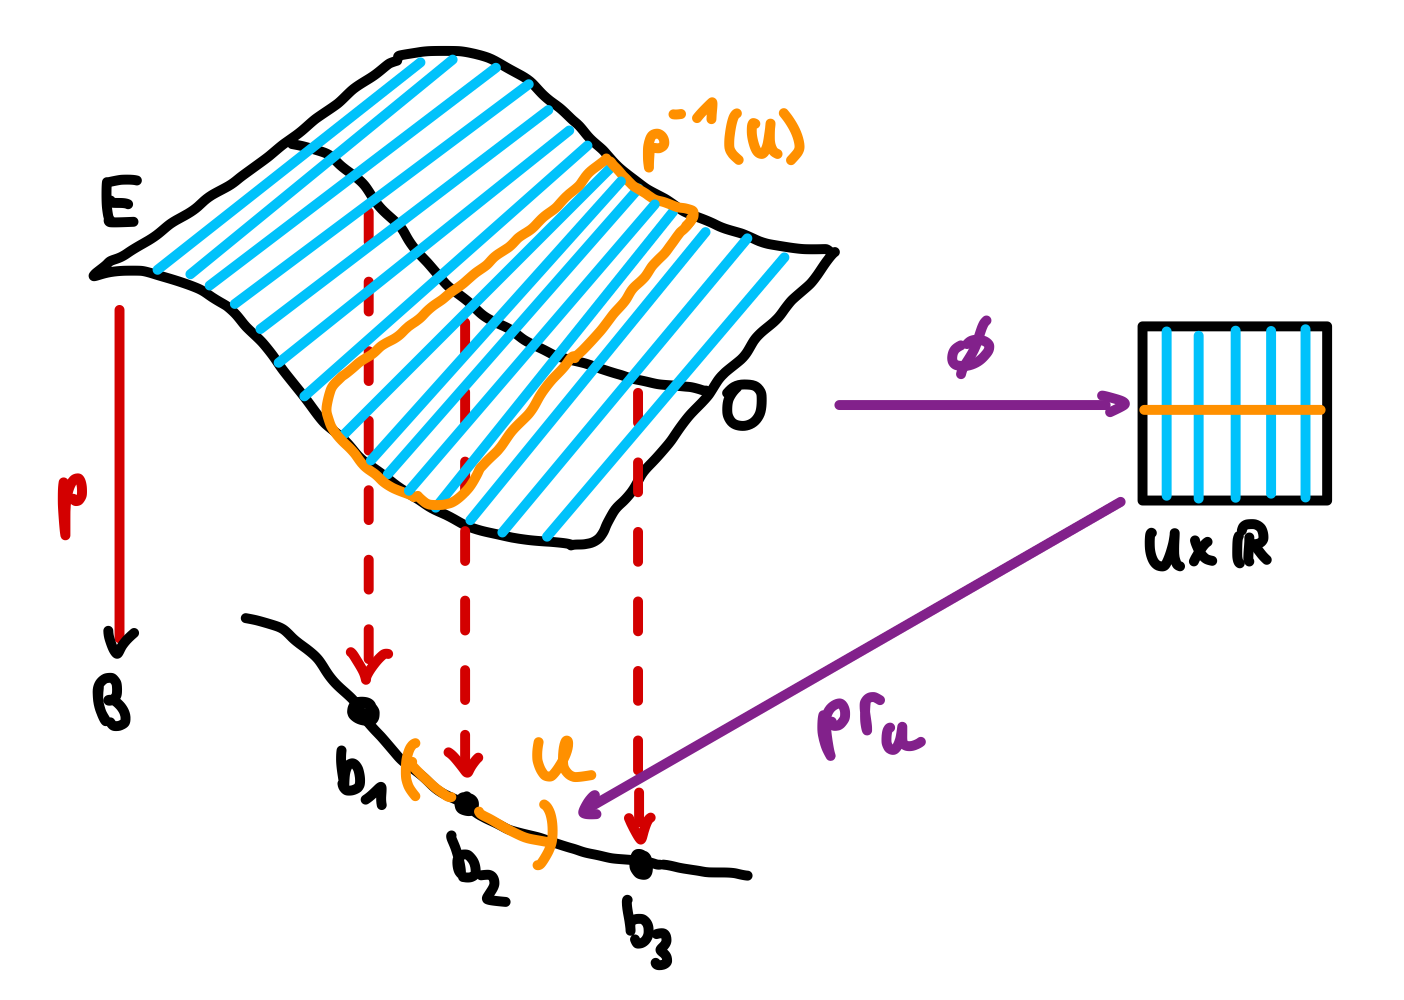
\includegraphics[width=0.3\linewidth]{Bilder/vektorbuendel.png}
\caption{Ein Vektorbündel.}
\end{figure}
\end{definition}
\begin{beispiele}Vektorbündel\\
\begin{enumerate}
\item Über jeder MFK $M$ gibt es das \textit{triviale Vektorbündel} von Rang $k$, gegeben durch
\begin{center}
\begin{tikzcd}
M \times \R^k \arrow[r, "p"] & M
\end{tikzcd}
\end{center}
mit $p(x, y) =x$.
\item Wir erinnern uns an die Definition vom $\R P^n$ als Raum der $1$-dim linearen UR im $\R^{n+1}$ und betrachten $E:= \{ (l, v) | l \in \R P^n, v \in l \} \sub \R P^n \times \R^{n+1}$. Mit der offensichtlichen Projektion $p: E \to  \R P^n$ ist $E$ ein Vektorbündel von Rang $1$ über $\R P^n$.
\begin{beweis}
Zuerst gilt es zu zeigen, dass $E \sub \R P^n \times \R^{n+1}$ eine UMF ist. Für den $\R P^n$ haben wir bereits Karten $U_i = \{ l \in \R P^n | \text{Projektion auf} \ i \text{-te Koordinate ist bijektiv}\}$ etabliert. $U_i$ wird parametrisiert durch die Abbildung $\psi_i : \R^n \to \R P^n, \ (x_1, \dots, x_n) \mapsto [(x_1, \dots, x_{i-1}, 1, x_i, \dots, x_n)]$. Das Urbild $p^{-1}(U_i)$ kann parametrisiert werden durch
\begin{align}
\rho_i: \R^n \times \R &\to \R P^n \times \R^{n+1} \\
(x, \lambda) &\mapsto \left( [(x_1, \dots, x_{i-1}, 1, x_i, \dots, x_n)], \lambda \cdot (x_1, \dots, x_{i-1}, 1, x_i, \dots, x_n)\right)
\end{align}
Das ist offenbar eine glatte Immersion, die $p^{-1}(U_i)=E \cap (U_i \times \R^{n+1})$ parametrisiert.
Aus dieser Karte für $E$ erhalten wir die lokalen Trivialisierungen über $U_i$:\\
$\phi_i: p^{-1}(U_i) \to U_i \times \R$ ist gegeben durch $(l, v) \mapsto (\psi_i \times \id_\R) \rho_i^{-1}(l,v)$.
\end{beweis}
\item Tangentialbündel einer UMF $M \sub \R^n$:\\
Mit unseren Konventionen ist $T_xM \sub \{x\} \times \R^n$ ein linearer UR der Dimension $k$. Damit ist dann $TM := \bigcup_{x \in M} T_xM$ eine Teilmenge von $M \times \R^n \sub \R^n \times \R^n$. Um Einzusehen, dass $TM \sub \R^n \times \R^n$ eine UMF ist, benutzen wir die Definition einer UMF als lokales Urbild einer Submersion.
\begin{beweis}
Sei $x\in M$ und sei $\psi: U \to \R^{n-k}$ eine auf einer offenen Umgebung $U$ von $x$ definierte Submersion mit $U \cap M = \psi^{-1}(0)$. Dann gilt für $y \in U \cap M$, dass $T_y M = \ker \psi_{\ast,y}$. Wir können also $TM \cap \left( (U \cap M) \times \R^n \right)$ beschreiben als Urbild von $0 \in \R^{n-k} \times \R^{n-k}$ unter der Abbildung:
\begin{align}
\Psi: U \times \R^n &\to \R^{n-k} \times \R^{n-k}\\
(z, v) &\mapsto \left( \psi(z), (\diff \psi)_z(v) \right).
\end{align}
Das Differential hat Blockform:
\begin{equation}
\diff \Psi_{(z,v)} = \mat{\diff \psi_z, 0}{\ast, \diff \psi_z},
\end{equation}
ist also surjektiv für alle $(z, v) \in U \times \R^n$. Weiterhin gilt
\begin{equation}
\Psi(z,v) = 0 \iff z \in M \wedge v \in T_zM,
\end{equation}
also allgemein $(z, v) \in TM \cap (U \times \R^n)$. Damit ist bewiesen, dass $TM \sub \R^n \times \R^n$ eine UMF der Dimension $2k$ ist.
\end{beweis}
Die Projektion $\pi: TM \to M$ ist als Einschränkung von $\R^n \times \R^n \to \R^n$ glatt, lokale Trivialisierungen erhält man aus der Beschreibung von $M$ über lokale Karten.
\end{enumerate}
\end{beispiele}
\begin{definition}{\textit{direkte Summe}}{direktesumme}
Seien $p_1: E_1 \to B$ und $p_2: E_2 \to B$ zwei Vektorbündel über der MFK $B$. Sei weiterhin $E:=p^{-1}(\Delta)\sub E_1 \times E_2$ das Urbild der Diagonalen $B \cong \Delta := \{(b,b)\ | \ b \in B \} \sub B \times B$. Dann heißt $E = E_1 \oplus E_2$ \textbf{direkte Summe} oder \textbf{Whitney-Summe} der Vektorbündel $E_1$ und $E_2$.\\ 
$(E,p,B)$ ist ein Vektorbündel über $B$ mit $p(e_1, e_2):=p_1(e_1)=p_2(e_2)$.
\end{definition}
\begin{bemerkung}Kozykelbedingung\\
Sei $p: E \to B$ ein Vektorbündel von Rang $k$ und seien $\phi: p^{-1}(U) \to U \times \R^k$ und $\psi: p^{-1}(V) \to V \times \R^k$ zwei lokale Trivialisierungen mit $U \cap V \neq \emptyset$.\\
Dann erhalten wir eine Übergangsabbildung
\begin{align}
\psi \circ \phi^{-1}: (U \cap V) \times \R^k &\to (U \cap V) \times \R^k \\
(b, v) &\mapsto (b, A_b(v)), \ A_b \in \text{GL}(k, \R).
\end{align}
Da $\psi \circ \phi^{-1}$ ein Diffeomorphismus, also insbesondere glatt, ist, ist auch $U \cap V \to \gl{k}{\R}, \ b \mapsto A_b$ glatt. Haben wir nun noch eine dritte Trivialisierung $\rho: p^{-1} (W) \to W \times \R^k$, so erhalten wir Übergangsabbildungen
\begin{align}
\rho \circ \psi^{-1}: (W \cap V) \times \R^k &\to (W \cap V) \times \R^k \\
(b, v) &\mapsto (b, B_b(v)) \\
\rho \circ \phi^{-1}: (W \cap U) \times \R^k &\to (W \cap U) \times \R^k \\
(b, v) &\mapsto (b, C_b(v))
\end{align}
für geeignete Abbildungen $B: W \cap V \to \gl{k}{\R}$ und $C: W \cap U \to \gl{k}{\R}$. Auf $U \cap V \cap W$ gilt $\rho \circ \phi^{-1} = (\rho \circ \psi^{-1})(\psi \circ \phi^{-1})$. Dadurch erhalten wir für $b \in U \cap V \cap W$ die \textbf{Kozykelbedingung}
\begin{equation}
C_b = B_b \circ A_b.
\end{equation}
\begin{figure}[H]
\label{fig:vektorbuendel}
\centering
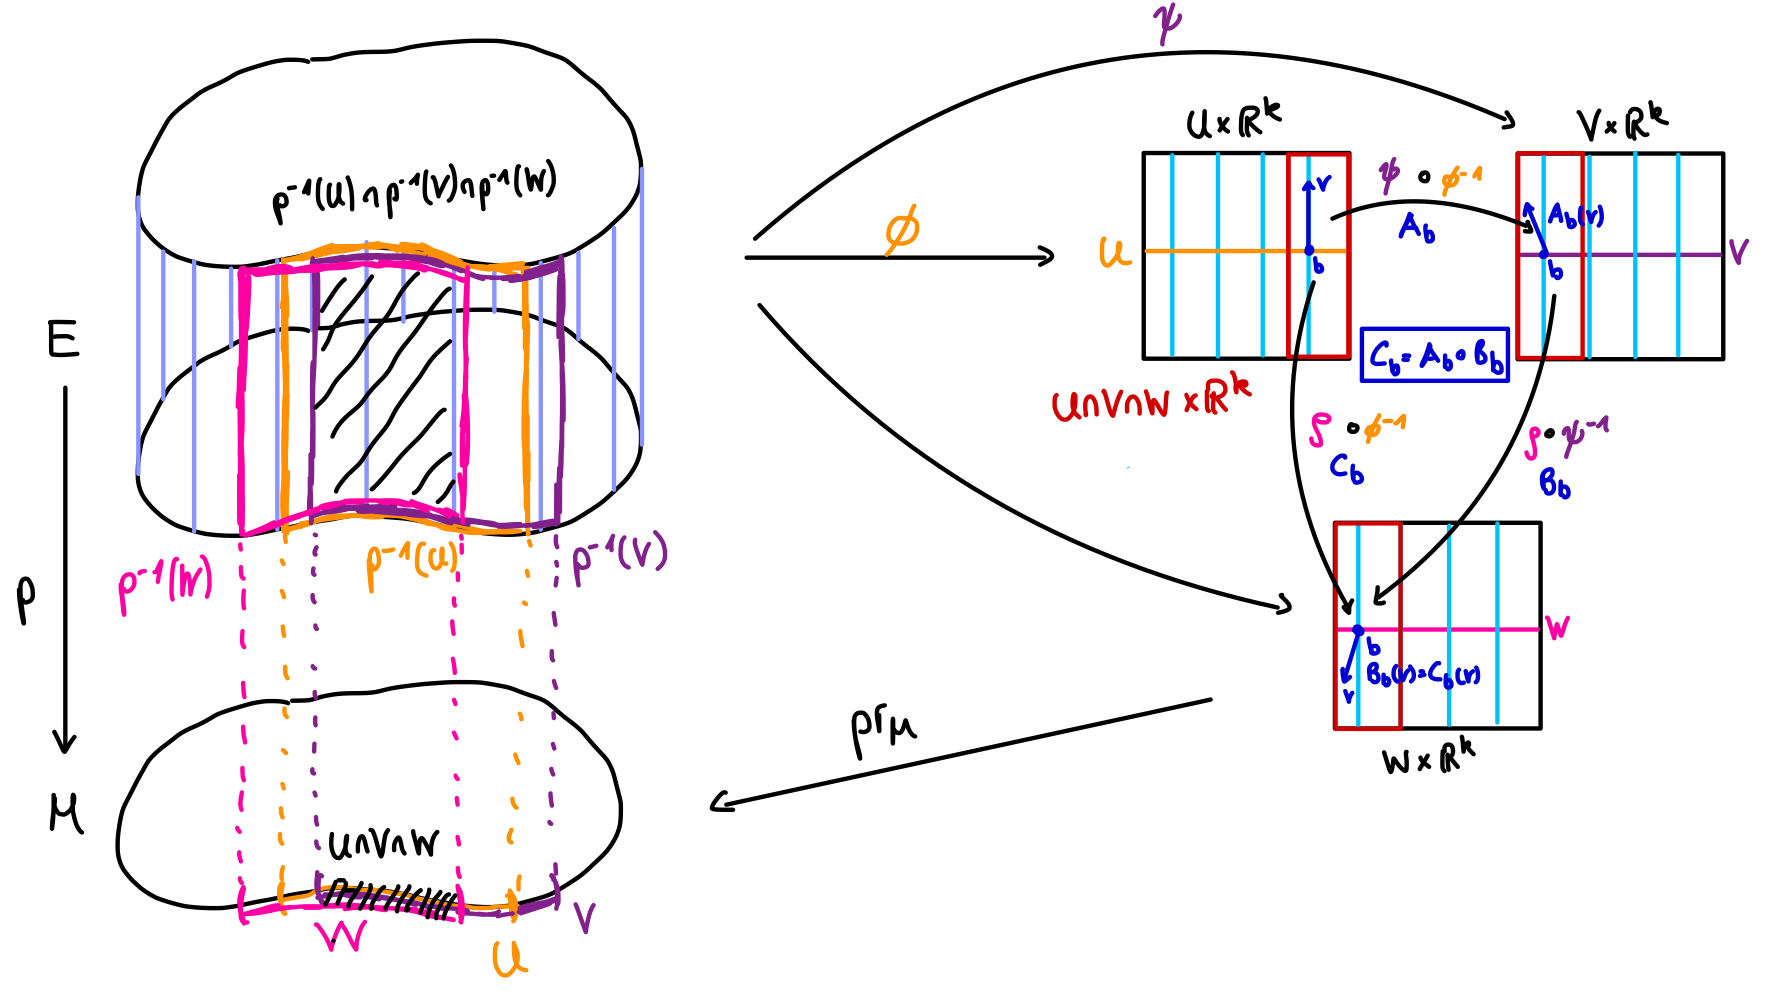
\includegraphics[width=0.5\linewidth]{Bilder/kozykel.png}
\caption{Eine Veranschaulichung der Kozykelbedingung für drei überlappende lokale Trivialisierungen.}
\end{figure}
Umgekehrt gilt Folgendes für die Konstruktion von Vektorbündeln:\\
Sei $B$ eine glatte MFK und $\{ U_\alpha \}_{\alpha  \in I}$ eine offene Überdeckung. Wir nehmen an, dass zu $\alpha, \beta \in I$ Abbildungen $\phi_{\alpha \beta}: U_\alpha \cap U_\beta \to \gl{k}{\R}$ gegeben sind, sodass für $\alpha, \beta, \gamma \in I$ die Kozykelbedingung
\begin{equation}
\left. \phi_{\alpha \gamma} \right|_{U_\alpha \cap U_\beta \cap U_\gamma} = \left. \left(\phi_{\alpha \beta} \circ \psi_{\beta \gamma} \right) \right|_{U_\alpha \cap U_\beta \cap U_\gamma}
\end{equation}
erfüllt ist. Aus diesen Daten konstruieren wir wie folgt ein Vektorbündel von Rang $k$ über $B$:\\
Auf $\amalg_{\alpha \in I} U_\alpha \times \R^k$ definieren wir eine Äquivalenzrelation durch $(x. v) \in U_\alpha \times \R^k \sim (x, w) \in U_\beta \times \R^k$ genau dann, wenn $\phi_{\alpha \beta}(w)=v$. Die Kozykelbedingung garantiert die Transitivität. Sei $E$ die Menge der Äquivalenzklassen dieser Relation $p: E \to B \ [(x,v)] \mapsto x$. Ist $U \sub U_\alpha$ Definitionsbereich einer Karte $h: U \to V \sub \R^k$ für $B$, dann ist 
\begin{align}
V \times \R^k &\to E \\
(y, v) &\mapsto [h^{-1}(y), v]
\end{align}
eine lokale Parametrisierung von $p^{-1}(U)$.
\begin{figure}[H]
\label{fig:vektorbuendel}
\centering
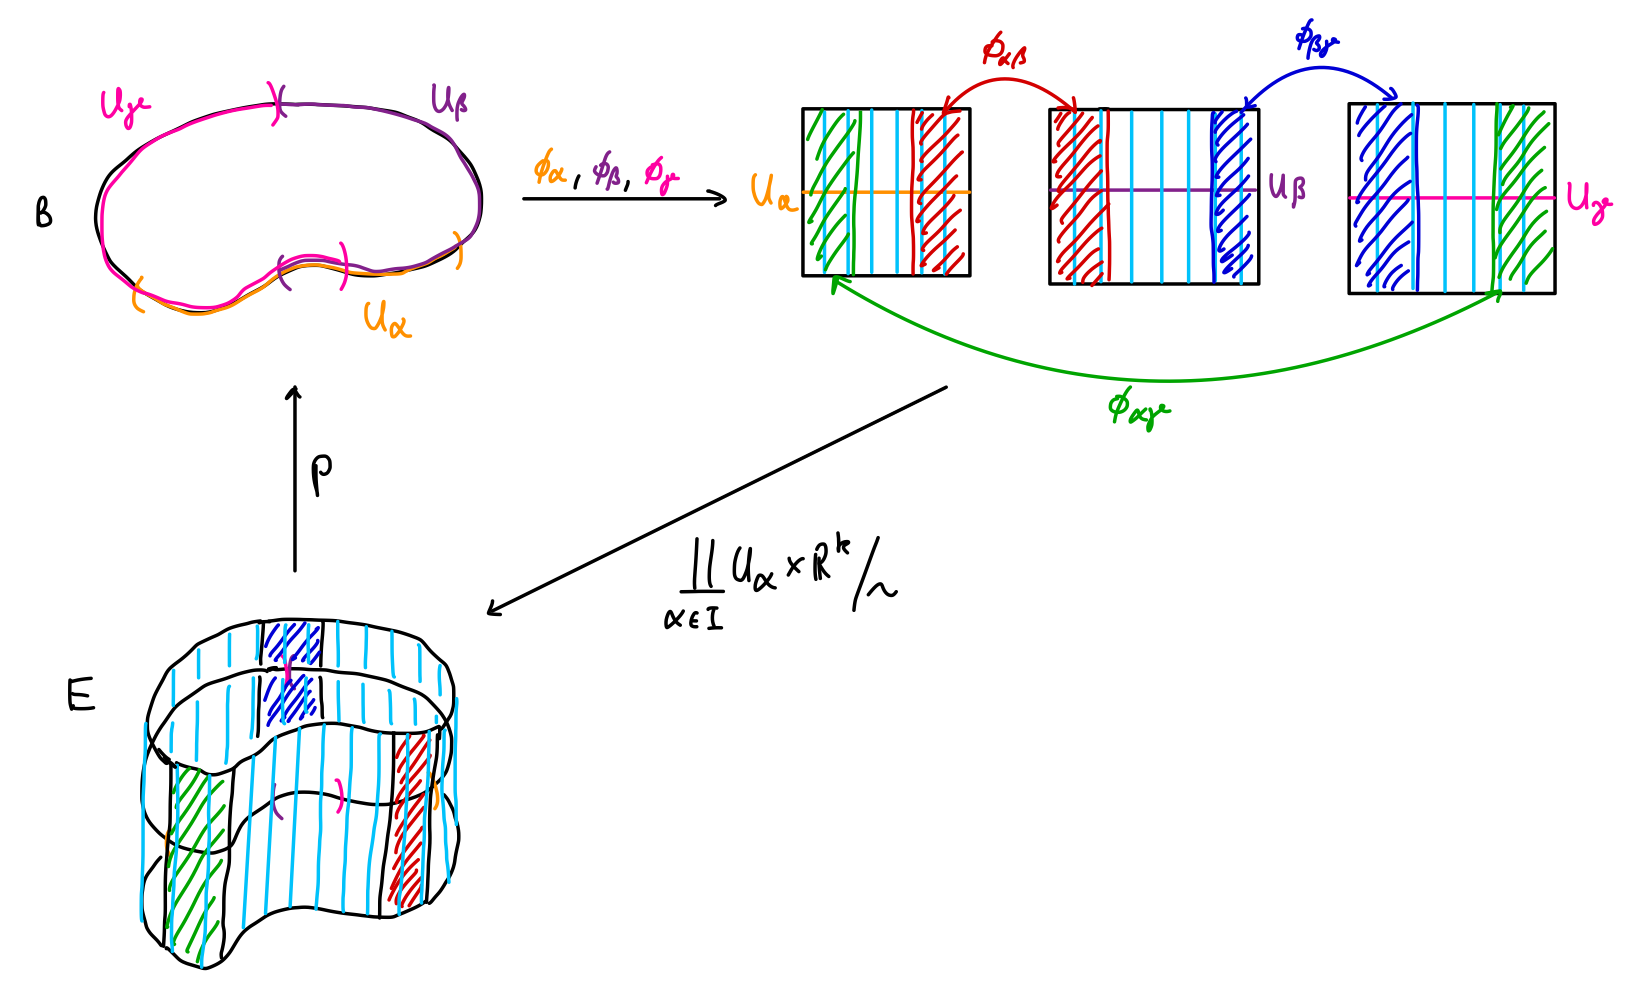
\includegraphics[width=0.5\linewidth]{Bilder/kozykelkonstrukt.png}
\caption{Drei lokale Trivialisierungen können mit Hilfe von Übergangsabbildungen, die die Kozykelbedingung erfüllen, verklebt werden, sodass ein Vektorbündel entsteht.}
\end{figure}
\end{bemerkung}
\begin{beispiele}
\begin{enumerate}
\item Wir betrachten $B = \sph^1 \sub \C$ mit $U_1 := \sph^1 \exc \{-1\}$ und $U_2 := \sph^1 \exc \{1\}$. Insbesondere ist dann $U_1 \cap U_2 = U_+ \cup U_-$. Weiterhin betrachten wir den Spezialfall $k=1$ und die Abbildung
\begin{align}
\phi_{12}: U_1 \cap U_2 &\to \gl{1}{\R} = \R \exc \{0\}\\
z &\mapsto \sgn (\Im (z)) = \begin{cases}
+1 \ \text{auf} \ U_+\\
-1 \ \text{auf} \ U_-
\end{cases}
\end{align}
Das mit diesen Daten konstruierte Bündel hat einen Totalraum, der diffeomorph zu einem offenen \textit{Möbiusband} ist.
\begin{figure}[H]
\label{fig:mobius}
\centering
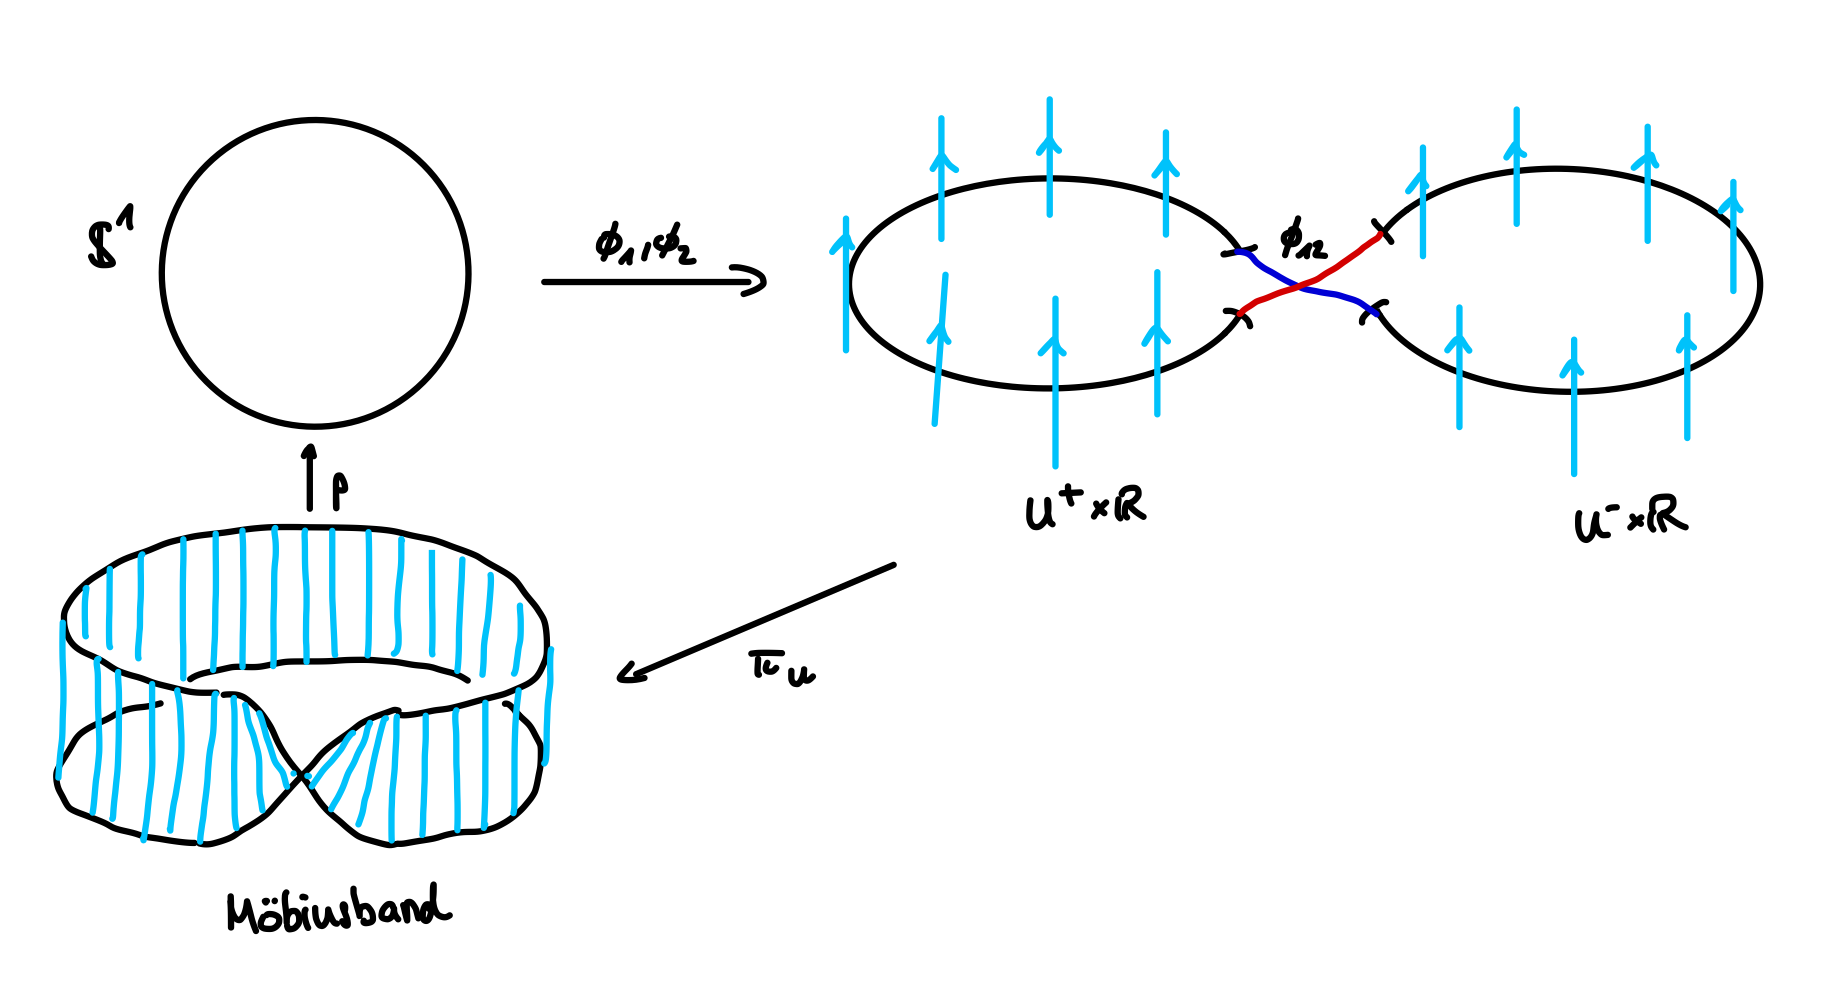
\includegraphics[width=0.4\linewidth]{Bilder/mobius.png}
\caption{Konstruktion des Möbiusbandes durch nichttriviale Verklebung.}
\end{figure}
\item Allgemeiner können wir $B= \sph^n$ mit den offenen Teilmengen $U_1 = \sph^n \exc \{(1,0, \dots, 0 ) \}$ und $U_2 = \sph^n \exc \{(-1, 0, \dots, 0 )\}$ betrachten. dann ist $U_1 \cup U_2 \cong \R^n \exc \{0\}$. Für gegebenes $k \in \N$ und eine glatte Abbildung
\begin{equation}
\rho: \R^n \exc \{0\} \to \gl{k}{\R}
\end{equation}
bestimmt $\rho$ ein Vektorbündel über $\sph^n$ von Rang $k$, indem man $U_1 \times \R^k$ und $U_2 \times \R^k$ über $U_1 \cap U_2 \times \R^k$ mit der Abbildung
\begin{align}
\Psi: (U_1 \cap U_2) \times \R^k &\to (U_1 \cap U_2) \times \R^k \\
(p,v) &\mapsto (p, \rho(p)v)
\end{align}
verklebt.\\
Konkret kann man ein solches $\rho: \R^n \exc \{0\} \to \gl{k}{\R}$ erhalten, indem man zu einer gegebenen Abbildung $\tilde{\rho}: \sph^{n-1} \to \gl{k}{\R}$ die Verknüpfung $\rho = \tilde{\rho} \circ \pi$ mit der Projektion
\begin{align}
\pi: \R^n \exc \{0\} &\to \sph^{n-1} \\
x &\mapsto \frac{x}{||x||}
\end{align}
betrachtet.\\
Für $n=k=2$ können wir mit $m \in \Z$ die Abbildung $\tilde{\rho}_m: \so{2} \cong \sph^1 \to \so{2} \sub \gl{2}{\R}, \ A \mapsto A^m$ betrachten. Auf diese Weise erhält man viele verschiedene Vektorbündel von Rang $2$ über $\sph^2$.  
\end{enumerate}
\end{beispiele}
Wir definieren den Isomorphiebegriff für Vektorbündel:
\begin{definition}{Bündelisomorphismus}{bundiso}
Seien 
\begin{tikzcd}
E_1 \arrow[r, "p_1"] & B_1
\end{tikzcd}
und 
\begin{tikzcd}
E_2 \arrow[r, "p_2"] & B_2
\end{tikzcd}
Vektorbündel. Ein \textbf{Bündelmorphismus} von $(E_1, p_1, B_1)$ zu $(E_2, p_2, B_2)$ besteht aus Abbildungen $f: B_1 \to B_2$ und $F: E_1 \to E_2$, sodass
\begin{center}
\begin{tikzcd}
E_1 \arrow[r, "F"] \arrow[d, "P_1"] & E_2 \arrow[d, "p_2"] \\
B_1 \arrow[r, "f"] & B_2
\end{tikzcd}
\end{center}
kommutiert und
\begin{equation}
F|_{(E_1)_b}: (E_1)_b \to (E_2)_{f(b)}
\end{equation}
linear ist für alle $b \in B_1$.
\end{definition}
\begin{definition}{Isomorphe Vektorbündel}{ismbund}
Zwei Bündel
\begin{tikzcd}
E_1 \arrow[r, "p_1"] & B
\end{tikzcd}
und 
\begin{tikzcd}
E_2 \arrow[r, "p_2"] & B
\end{tikzcd}
über derselben Basis heißen \textbf{isomorph}, falls ein Bündelisomorphismus $(F, f=\id)$ existiert, sodass $F_b: (E_1)_b \to (E_2)_b$ für alle $b \in B$ ein Isomorphismus ist.
\end{definition}
Nach diesem kleinen Exkurs wenden wir uns Tangentialbündeln zu. Das Tangentialbündel an eine glatte MFK $M$ kann man auch durch Verkleben aus lokalen ''Stücken'' erhalten:\\
Zunächst haben wir:
\begin{center}
\begin{tikzcd}
T\R^n = \R^n \times \R^n \arrow[r, "\pi = pr_1"] & \R^n.
\end{tikzcd}
\end{center}
Für $V \sub \R^n$ offen gilt $TV = \pi^{-1}(V) = V \times \R^n$. Ist jetzt $M$ eine glatte MFK der Dimension $n$, so wählen wir einen Atlas $\Af = \{(U_\alpha, \phi_\alpha)\}_{\alpha \in I}$. In unserer ersten Beschreibung von Tangentialräumen hatten wir Tangentialvektoren der Äquivalenzklasse von Tangentialvektoren in Karten definiert. Insbesondere erhalten wir also eine Parametrisierung von 
\begin{align}
\bigcup_{x \in U_\alpha} T_xM &\cong V_\alpha \times \R^n \\
[\phi_\alpha (y, v)] &\mapsfrom (y, v).
\end{align}
Ist $\phi_\beta: U_\beta \to V_\beta \sub \R^n$ eine andere Karte, so ist auf $W=U_\alpha \cap U_\beta$ die Übergangsabbildung
\begin{align}
\psi_{\alpha \beta}: V_\beta \times \R^n \supseteq W \times \R^n &\to W \times \R^n \sub V_\alpha \times \R^n \\
(x, v) &\mapsto \left( x, (\phi_\alpha \circ \phi_\beta^{-1})_{\ast, \phi_\beta(x)} (v) \right).
\end{align}
Aus der Kettenregel folgt, dass diese Übergänge zwischen lokalen Trivialisierungen tatsächlich die Kozykelbedingung erfüllen.\\
Verklebt man also 
$\bigsqcup_{\alpha \in I} U_\alpha \times \R^n$ mit Hilfe der Abbildungen $\psi_{\alpha \beta}$ von oben, erhält man das Tangentialbündel
\begin{tikzcd}
TM \arrow[r, "\pi"] & M.
\end{tikzcd}
\begin{figure}[H]
\label{fig:tangentialbund}
\centering
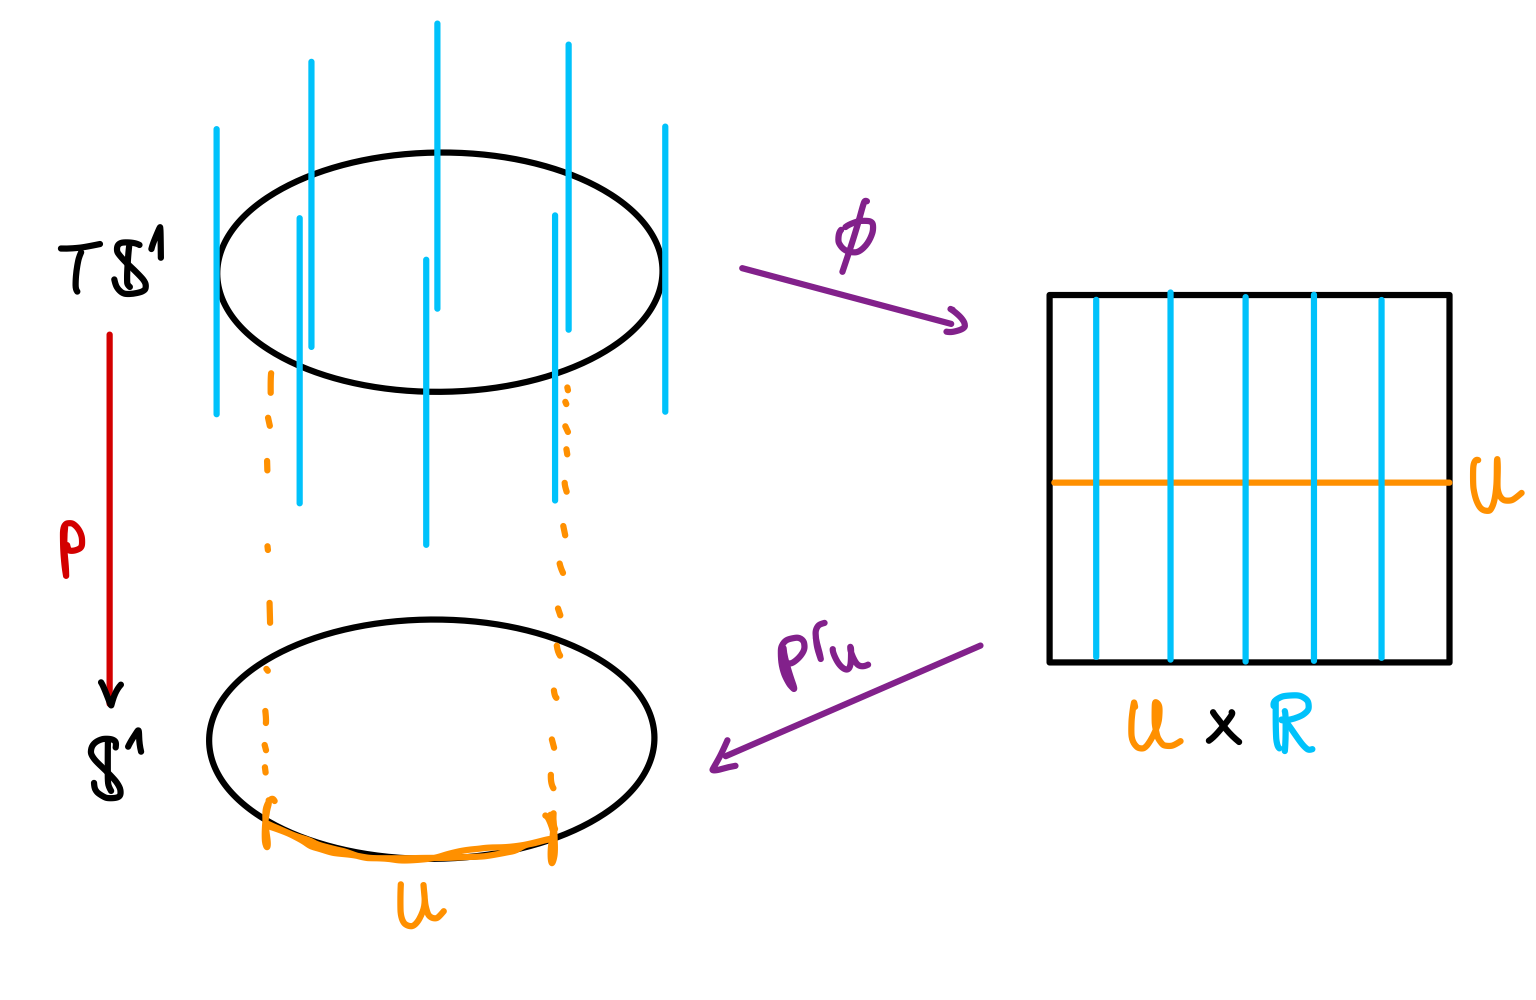
\includegraphics[width=0.4\linewidth]{Bilder/tangentialbundel.png}
\caption{Das Tangentialbündel der Sphäre $\sph^1$ mit lokaler Trivialisierung.}
\end{figure}
\begin{beispiel}Bündelmorphismus\\
Sei $f: M \to N$ eine glatte Abbildung. Dann ist $f_\ast:TM \to TN$ zusammen mit $f$ ein Bündelmorphismus:
\begin{center}
\begin{tikzcd}
TM \arrow[r, "f_\ast"] \arrow[d, "\pi"] & TN \arrow[d, "\pi"] \\
M \arrow[r, "f"] & N
\end{tikzcd}
\end{center}
\end{beispiel}
\begin{definition}{glatter Schnitt}{schnitt}
Sei $p: E \to B$ ein glattes Vektorbündel. Ein \textbf{glatter Schnitt} in $E$ ist eine glatte Abbildung 
\begin{equation}
s: B \to E
\end{equation}
mit $p \circ s = \id_B$.\\
Wir bezeichnen die Menge der Schnitte von $E$ als $\Gamma(E)$.
\begin{figure}[H]
\label{fig:schnitt}
\centering
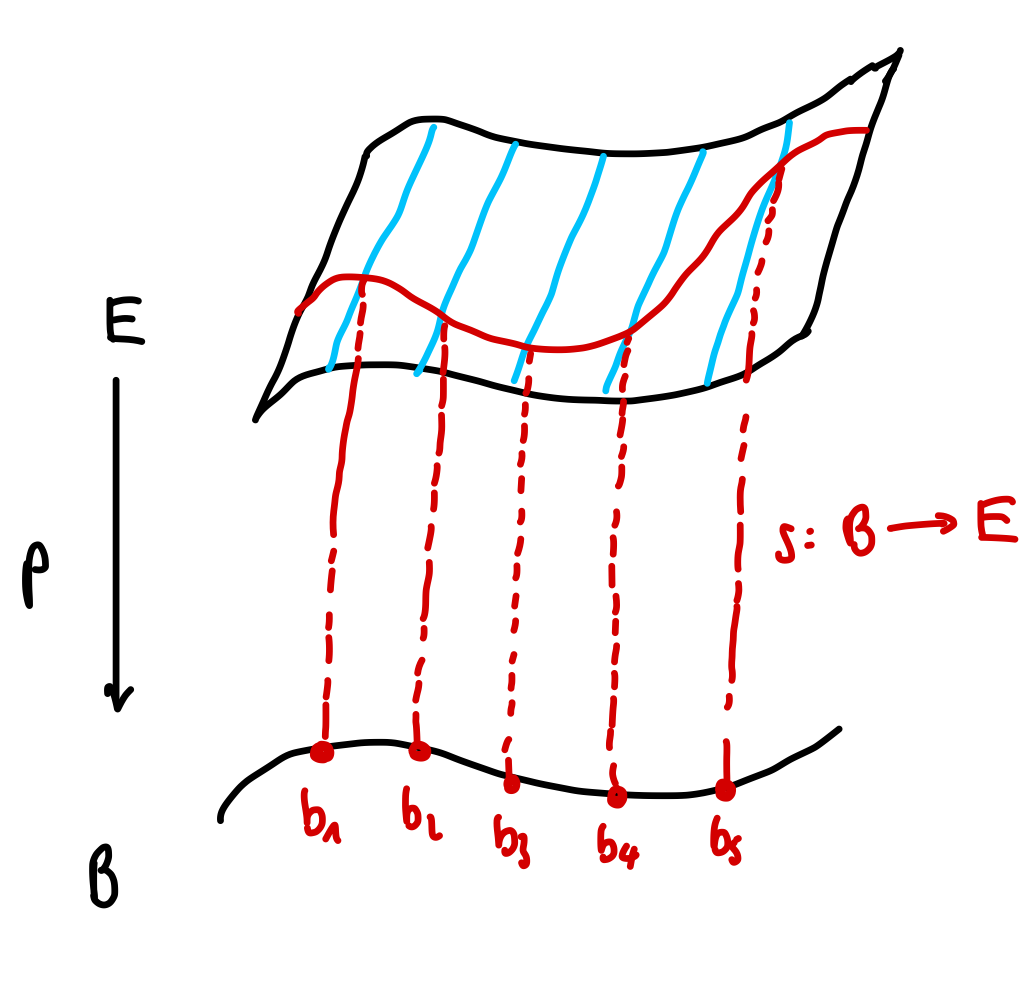
\includegraphics[width=0.3\linewidth]{Bilder/schnitt.png}
\caption{Mehrere Schnitte $s$ wählen zu $b_i$ Vektoren aus $E$ aus.}
\end{figure}
\end{definition}
Ein Schnitt wählt also auf glatte Weise zu jedem $b \in B$ einen Vektor $s(b) \in E_b$ aus. \footnote{Die begriffliche Ähnlichkeit zu Dedekind-Schnitten ist rein zufällig.}
\begin{bemerkungen}Nullschnitt und Vektorraum\\
\begin{enumerate}
\item In jedem Vektorbündel gibt es einen kanonischen Schnitt, der jedem Punkt $b \in B$ den Ursprung des Vektorraums $E_b$ zu. Diesen Schnitt nennt man den \textbf{Nullschnitt} des Bündels.
\item Sind $s_1, s_2 \in \Gamma (E)$, so ist 
\begin{equation}
(s_1+s_2)(b):=s_1(b)+s_2(b)
\end{equation}
wieder ein Schnitt, und für $s \in \Gamma (E)$ und $\lambda \in \R$ ist auch 
\begin{equation}
(\lambda s)(b) := \lambda s(b)
\end{equation}
ein Schnitt. Mit diesen Operationen wird $\Gamma(E)$ zu einem reellen VR.
\item Etwas allgemeiner ist auch für $s \in \Gamma (E)$ und $f \in \cinf{B}{}$ durch
\begin{equation}
(f \cdot s)(b) := f(b) \cdot s(b)
\end{equation}
auch wieder ein Schnitt definiert. Auf diese Weise wird $\Gamma (E)$ zu einem \textit{Modul} über dem Ring $\cinf{B}{}$.
\end{enumerate}
\end{bemerkungen}
\begin{definition}{Vektorfelder}{vekfeld}
(Glatte) Schnitte im Tangentialbündel 
\begin{tikzcd}
TM \arrow[r, "\pi"] & M.
\end{tikzcd}
einer glatten MFK $M$ nennt man \textbf{glatte Vektorfelder auf} $M$.
\begin{figure}[H]
\label{fig:vektorfeldaustang}
\centering
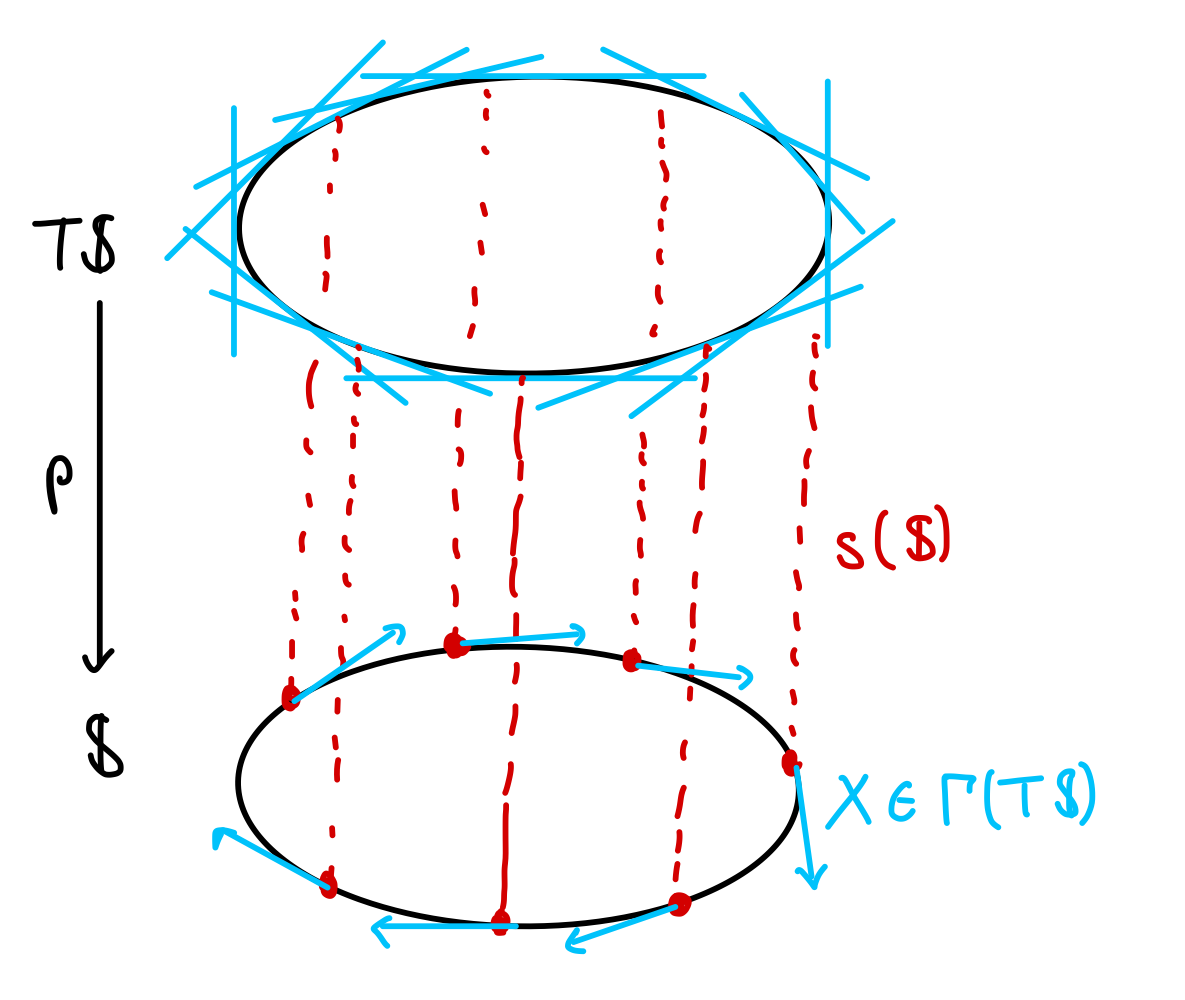
\includegraphics[width=0.3\linewidth]{Bilder/vektorfeldsph.png}
\caption{Aus dem Tangentialbündel von $\sph$ wird ein Vektorfeld ausgewält.}
\end{figure}
\end{definition}
\begin{bemerkung}
Ist $p: E \to B$ ein Vektorbündel und $S \sub B$ eine UMF, so ist
\begin{equation}
p|_{p^{-1}(S)}: p^{-1}(S) (=: E|_S) \to S
\end{equation}
auch ein glattes Vektorbündel.
\end{bemerkung}
\begin{beispiel}
Ist $U \in M$ offen, so gilt $TM|_U = TM$. Hat $S \in M$ positive \textit{Kodimension} (d.h. $\dim S < \dim M$), dann sind die Vektorbündel $TM|_S$ und $TS$ verschieden (da ihr Rang verschieden ist).
\end{beispiel}
Sei $M$ eine glatte MFK und $\phi: U \to V \sub \R^n$ eine lokale Karte mit Koordinaten $(x_1, \dots, x_n)$. Dann definiert die Zuordnung
\begin{align}
\frac{\partial}{\partial x_i}: U &\to TM|_U = TU \\
p &\mapsto \frac{\partial}{\partial x_i}|_p
\end{align}
für jedes $i \in \{1, \dots, n \}$ ein glattes, lokales (d.h. auf $U$ definiertes) Vektorfeld. In der durch die Karte $\phi: U \to V$ bestimmten lokalen Trivialisierung
\begin{equation}
\psi: TM|_U \to TV = V \times \R^n
\end{equation}
entspricht $\frac{\partial}{\partial x_i}$ dem konstanten Vektorfeld
\begin{equation}
p \mapsto \left( \phi(p), (0, \dots, 1, 0, \dots, 0)\right).
\end{equation}
In jedem $p \in U$ bilden die Vektoren $\frac{\partial}{\partial x_1}|_p, \dots, \frac{\partial}{\partial x_n}|_p$ eine Basis von $T_pM$. Es ist dann klar, dass jedes auf $U$ definiertes Vektorfeld sich als Linearkombination der $\frac{\partial}{\partial x_i}$ mit Koeffizienten in $\mathcal{C}^\infty (M)$ schreiben lässt.
\begin{satz}{}{}
Sei $\phi: U \to V \sub \R^n$ eine Karte für $M$ mit lokalen Koordinaten $(x_1, \dots, x_n)$. Dann hat jedes lokal definierte, glatte Vektorfeld $X \in \Gamma(TM|_U)$ die Darstellung
\begin{equation}
X(p) = \Sum{i,1,n} X(x_i) \cdot \left.\frac{\partial}{\partial x_i}\right|_p \ (\ast)
\end{equation}
mit der Derivation $X_p(x_i) =: X(x_i)(p)$ im Punkt $p$.\\
Umgekehrt wird für beliebige Funktionen $f_1, \dots, f_n \in \cinf{U}{}$ durch
\begin{equation}
fX := \Sum{i,1,n} f_i \frac{\partial}{\partial x_i}
\end{equation}
ein glattes, lokales Vektorfeld definiert.
\begin{figure}[H]
\label{fig:normalformvek}
\centering
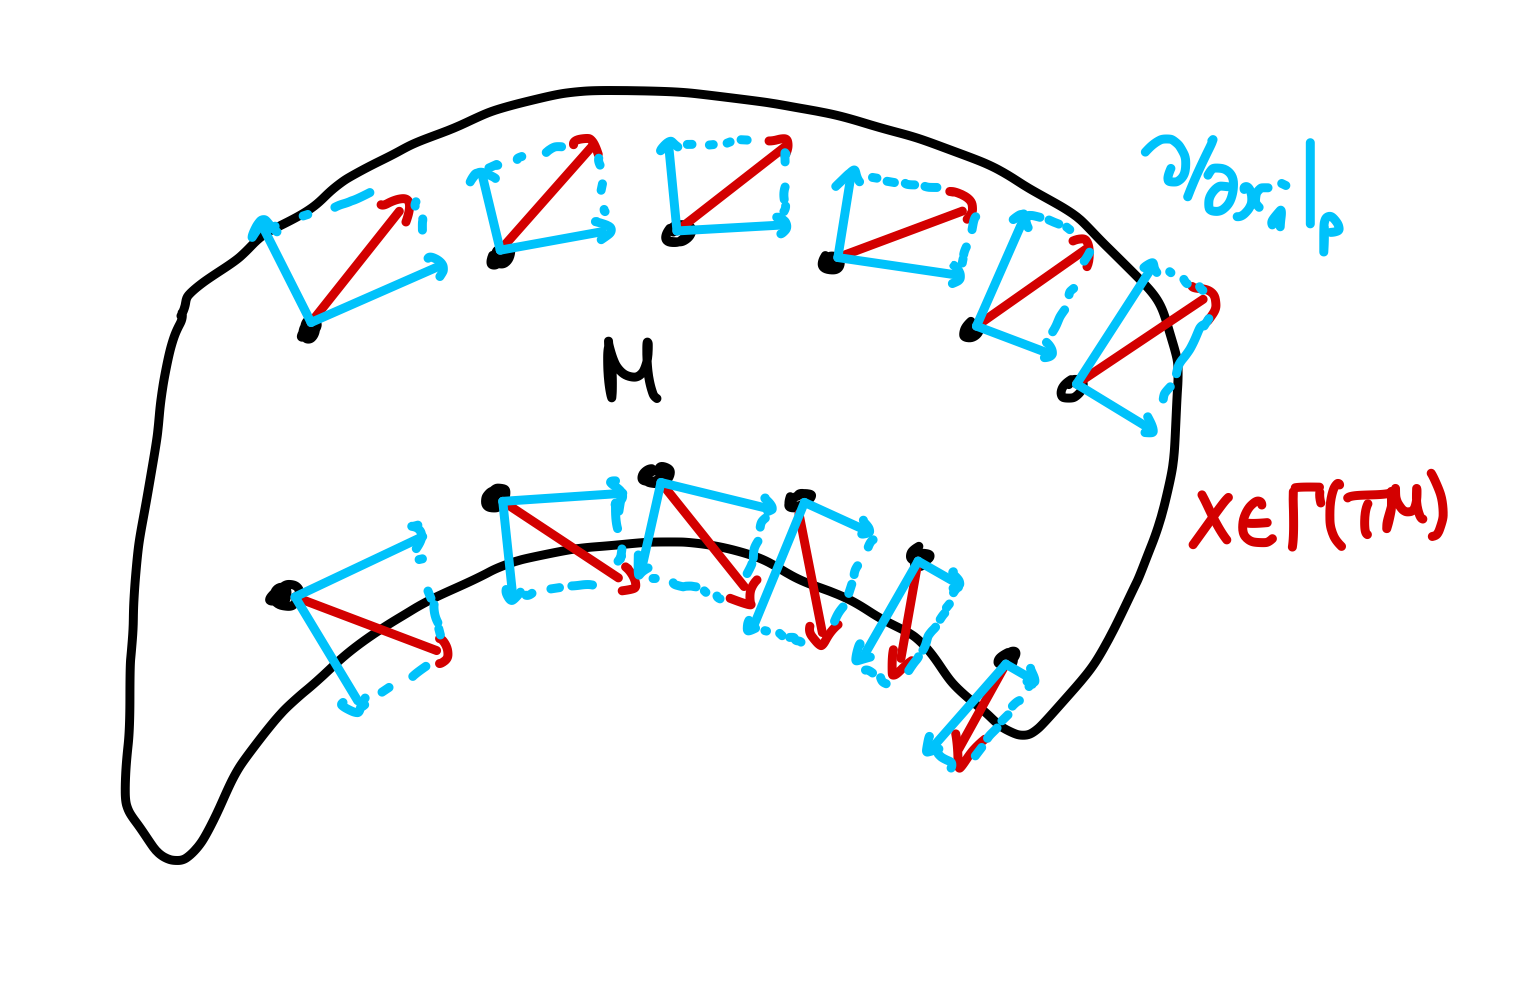
\includegraphics[width=0.25\linewidth]{Bilder/normalformvek.png}
\caption{Die Normalform eines Vektorfeldes.}
\end{figure}
\end{satz}
\begin{beweis}
Die punktweise Formel $(\ast)$ hatten wir uns bereits überlegt, als wir über Tangentialvektoren als punktweise Derivationen gesprochen haben.\\
Die Funktionen $X(x_i)$ sind glatt, weil sie die Darstellung von $X$ in der lokalen Trivialisierung durch $\left( \frac{\partial}{\partial x_1}, \dots, \frac{\partial}{\partial x_n} \right)$ beschreiben.\\
Die letzte Aussage ist offensichtlich.
\end{beweis}
\begin{bemerkungen}
\begin{enumerate}
\item Ist $p: E \to B$ ein Vektorbündel von Rang $k$, $U \in B$ eine offene Menge und $s_1, \dots, s_k: U \to E|_U$ Schnitte von $E$ über $U$, sodass in jedem Punkt $b \in U$ die Vektoren $s_1(b), \dots, s_k(b)$ eine Basis der Faser $E_b$ bilden, so nennt man $(s_1, \dots, s_k)$ einen \textbf{lokalen Rahmen} für $E$.\\
Jede lokale Trivialisierung gibt einen solchen lokalen Rahmen, und umgekehrt bestimmt auch jeder lokale Rahmen für $E$ eine lokale Trivialisierung von $E$.
\item Man nennt ein Vektorbündel \textbf{trivial}, falls ein globaler Rahmen existiert, d.h. falls es isomorph zum Bündel $B \times \R^k \to B$ ist.
\end{enumerate}
\end{bemerkungen}
\begin{bemerkung}
Zu jeder Konstruktion mit Vektorräumen gibt es eine zugehörige Konstruktion mit Vektorbündeln über einer festen Basis.
\begin{beispiel}
Jeder Vektorraum hat einen Dualraum (und lineare Abbildungen $L: V \to W$ induzieren duale Abbildungen $L^\ast: W \to V$). Analog kann man für jedes Vektorbündel 
\begin{tikzcd}
E \arrow[r, "p"] & B
\end{tikzcd}
ein duales Bündel 
\begin{tikzcd}
E^\ast \arrow[r, "p"] & B
\end{tikzcd}
konstruieren, sodass $(E^\ast)_b = (E_b)^\ast$ gilt. Wendet man diese Überlegungen auf $TM \to M$ an, so erhält man das \textit{Kotangentialbündel} $T^\ast M \to M$.\\
 Dual zur lokalen Basis von Vektorfeldern $\left( \frac{\partial}{\partial x_1}, \dots, \frac{\partial}{\partial x_n}\right)$ hat man eine lokale Basis von $1$-Formen $\left( dx_1, \dots, dx_n \right)$.\\
Dual zum Differential $f_\ast: TM \to TN$ einer Abbildung $f: M \to N$ erhalten wir $f^\ast: T^\ast N \to T^\ast M$ (Zurückziehen von $1$-Formen).
\end{beispiel}
\end{bemerkung}
\begin{definition}{Algebra}{alg}
Eine \textbf{Algebra über} $\R$ ist ein $\R$-Vektorraum $A$ mit einer Multiplikation
\begin{equation}
\cdot: A \times A \to A,
\end{equation}
die bilinear ist, es gilt also
\begin{gather}
(a_1 + a_2) \cdot b = a_1b + a_2b \\
a(b_1+b_2) = ab_1 + ab_2\\
\forall \lambda \in \C (\lambda a)b = \lambda (ab) = a \cdot (\lambda b).
\end{gather}
\end{definition}
\begin{bemerkung}
Mit punktweiser Addition ist der Raum $\cinf{M}{\R}$ ein $\R$-Vektorraum. Mit der punktweisen Multiplikation wird dieser zu einer Algebra über $\R$.
\end{bemerkung}
\begin{definition}{Derivation reloaded}{dervneu}
Eine \textbf{Derivation} auf $A$ ist eine $\R$-lineare Abbildung
\begin{equation}
\Df: A \to A
\end{equation}
mit $\Df (ab) = \Df (a) b + a \Df (b)$.\\
Die Derivationen auf $A$ bilden einen reellen Vektorraum $\der{p}$.
\end{definition}
\begin{satz}{Isomorpie von $\Gamma$ und $\text{Der} (\text{C}^\infty)$}{isomorphveccinf}
Sei $M$ eine glatte MFK. Der reelle Vektorraum der Vektorfelder $\Gamma (TM)$ auf $M$ ist auf natürliche Weise\footnote{Natürlich heißt, dass wir keine konkrete, nicht-kanonische Wahl für den Isomorphismus treffen müssen.} isomorph zum Vektorraum $\text{Der}(\cinf{M})$.
\end{satz}
\begin{beweis}
Da Vektorfelder punktweise Tangentialvektoren sind, wird für $X \in \Gamma (TM)$ und $f \in \cinf{M}$ durch
\begin{equation}
(Xf)(p):= \underbrace{X_p}_{\in T_pM} f
\end{equation}
eine Funktion $Xf: M \to \R$ definiert. In lokalen Koordinaten rechnet man leicht nach, dass diese Funktion glatt ist. Dazu nutzt man die Darstellung $X=\sum_i X_i \frac{\partial}{\partial x_i}$ und wendet sie auf $f$ an, was eine Summe glatter Funktionen liefert.\\
Außerdem ist die Zuordnung
\begin{align}
\cinf{M} &\to \cinf{M} \\
f &\mapsto Xf
\end{align}
linear über $\R$, d.h. für $\lambda, \mu \in \R$ und $f, g \in  \cinf{M}$ gilt $X(\lambda f + \mu g)=\lambda X f + \mu X g$. Auch die Leibnizregel $X(f \cdot g)= (Xf) \cdot g + f \cdot (Xg)$ ist erfüllt. Also wird auf diese Weise jedem Vektorfeld $X \in \Gamma (TM)$ eine Derivation $\Df_x \in \text{Der} (\cinf{M})$ zugeordnet, nämlich $\Df_X (f) = Xf$. Die Abbildung $\Gamma (TM) \to \text{Der} (\cinf{M})$ ist offensichtlich linear.\\
Ist umgekehrt $\Df \in \text{Der} (\cinf{M})$, so erhalten wir durch Auswertung in $p \in M$ einen Tangentialvektor $X_\Df (p) \in \der{p} \cong T_pM$. Diese Zuordnung definiert einen Schnitt
\begin{align}
M &\to TM \\
p &\mapsto X_\Df (p).
\end{align}
Da $\Df f$ für alle $f \in \cinf{M}$ wieder glatt ist, gilt dies insbesondere auch für (geeignet abgeschnittene) lokale Koordinatenfunktionen $x_i$. Also hat $X_\Df$ die lokale Darstellung
\begin{equation}
X_\Df |_U = \Sum{i,1,n} \Df (x_i) \frac{\partial}{\partial x_i}
\end{equation}
mit glatten Koeffizienten $\Df (x_i)$. Also ist $X_D$ ein glattes Vektorfeld.\\
Da diese beiden Abbildungen offensichtlich invers zueinander sind, sind sie Isomorphismen zwischen $\Gamma (TM)$ und $\text{Der} (\cinf{M})$.
\end{beweis}
Wir nutzen hier eine sehr abstrakte Sichtweise, da wir dadurch eine zusätzliche algebraische Struktur auf $\Gamma (TM)$ erhalten. Dazu erst ein paar algebraische Vorüberlegungen:
\begin{bemerkung}
Ist $A$ eine $\R$-Algebra und $\Df_1, \Df_2 \in \text{Der}(A)$, so gilt:
\begin{align}
\Df_1 \Df_2 (ab) &= \Df_1 (\Df_2 (a)b+ a \Df_2(b))\\
&=(\Df_1 \Df_2 (a))b + \Df_2(a)\cdot \Df_2(b) + \Df_1 (a) \cdot \Df_2 (b) + a (\Df_1 \Df_2 (b))
\end{align}
Wir beobachten, dass $\Df_1 \Df_2$ \textit{keine} Derivation ist, aber die Störterme symmetrisch in $\Df_1$ und $\Df_2$ sind.
\end{bemerkung}
\begin{definition}{Kommutator}{komm}
Für $\Df_1, \Df_2 \in \text{Der} (A)$ ist der \textbf{Kommutator} gegeben durch
\begin{equation}
[\Df_1, \Df_2] := \Df_1 \Df_2 - \Df_2 \Df_1.
\end{equation}
\end{definition}
Der Kommutator ist also für $\Df_1, \Df_2 \in \text{Der} (A)$ wieder eine Derivation.
\begin{satz}{Kommutator als Lie-Algebra}{liederp}
Sei $A$ eine $\R$-Algebra. Dann ist $\text{Der} (A)$ mit dem Kommutator
\begin{equation}
[., .]: \text{Der} (A) \times \text{Der} (A) \to \text{Der} (A),
\end{equation}
auch \textbf{Lie-Klammer} genannt, eine \textit{Lie-Algebra}. Es gilt somit:
\begin{itemize}
\item $[., .]$ ist $\R$-bilinear.
\item $[., .]$ ist \textit{schiefsymmetrisch}: $ [ \Df_2, \Df_1] = - [\Df_1, \Df_2 ]$.
\item Es gilt die \textit{Jacobi-Identität}: $[\Df_1, [\Df_2, \Df_3]] + [\Df_2, [\Df_3, \Df_1]] + [\Df_3, [\Df_1, \Df_2]] = 0$.
\end{itemize}
\end{satz}
\begin{beweis}
Die ersten beiden Bedingungen folgen direkt aus der Definition. Für die dritte Bedingung muss man nachrechnen: $[\Df_1, [\Df_2, \Df_3]] = [\Df_1, \Df_2\Df_3-\Df_3\Df_2]$. Also gilt
\begin{align}
[\Df_1, [\Df_2, \Df_3]] &= \Df_1\Df_2\Df_3 - \Df_2\Df_3\Df_1-\Df_1\Df_3\Df_2 + \Df_3\Df_2\Df_1\\
[\Df_2, [\Df_3, \Df_1]] &= \Df_2\Df_3\Df_1 - \Df_3\Df_1\Df_2-\Df_2\Df_1\Df_3 + \Df_1\Df_3\Df_2.
\end{align}
\end{beweis}
\begin{korollar}{Glatte VF als Lie-Algebra}{gvflie}
Auf jeder glatten MFK $M$ bilden die glatten Vektorfelder $\Gamma (TM)$ mit dem Kommutator eine Lie-Algebra.
\end{korollar}
\begin{beweis}
Für lokale Koordinatenvektorfelder $\fracpart{x}, \frac{\partial}{\partial x_j}$ gilt
\begin{equation}
\left[ \fracpart{x}, \frac{\partial}{\partial x_j} \right] =0.
\end{equation}
Übung (A12).
\end{beweis}
\begin{satz}{Differential und Lie-Klammer}{difflieklammer}
Seien $M, N$ glatte MFK und $F: M \to N$ eine glatte Abbildung. Gilt für $X_1, X_2 \in \Gamma(TM)$ und $\bar{X}_1, \bar{X}_2$ an jedem Punkt $p \in M$ die Beziehung
\begin{equation}
(\bar{X}_i)_{F(p)} = F_\ast (X_i)_p,
\end{equation}
so gilt auch
\begin{equation}
[\bar{X}_1, \bar{X}_2]_{F(p)} = F_\ast [X_1, X_2]_p
\end{equation}
für alle $p \in M$.
\end{satz}
\begin{beweis}
Übung (A12)
\end{beweis}
\begin{definition}{Integralkurve}{intkurv}
Sei $M$ eine glatte MFK und $X \in \Gamma (TM)$ ein glattes Vektorfeld.\\
Eine Kurve $c: [a,b] \to M$ heißt \textbf{Integralkurve} für $X$, falls für alle $t \in (a,b)$ gilt:
\begin{equation}
\dot{c}(t) = X_{c(t)}.
\end{equation}
\begin{figure}[H]
\label{fig:integralkurve}
\centering
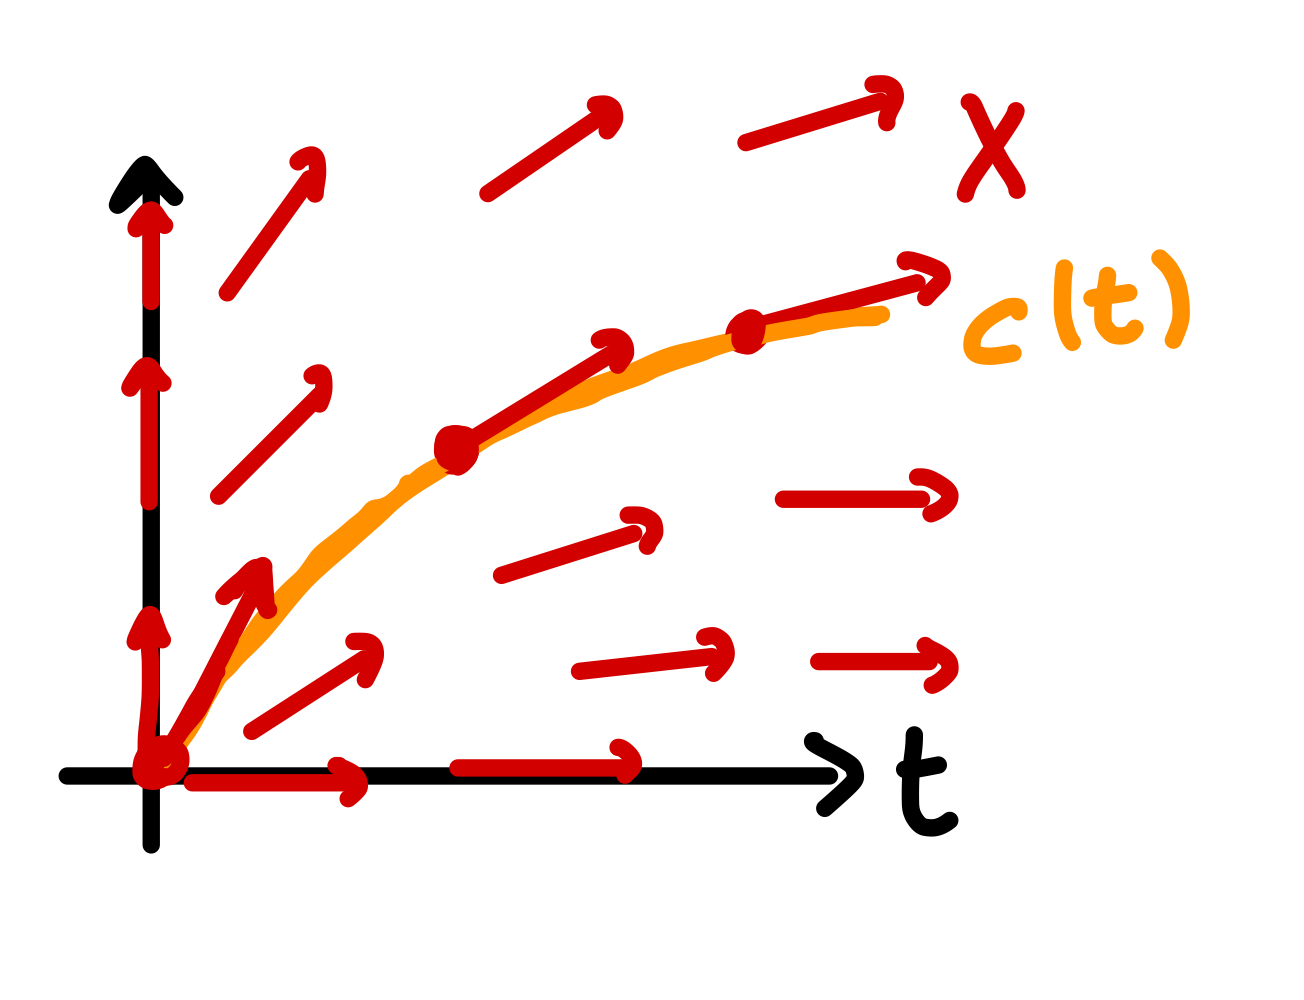
\includegraphics[width=0.25\linewidth]{Bilder/integralkurve.png}
\caption{Eine Integralkurve $c(t)$ eines Vektorfeldes $X$.}
\end{figure}
\end{definition}
In lokalen Koordinaten nahe $c(t_0) \in M$ wird diese Bedingung zu einer gewöhnlichen DGL 1. Ordnung für die Koordinaten der Kurve.
\begin{bemerkung}
Aus der allgemeinen Theorie der Differentialgleichungen erhalten wir zu jedem $p \in M$ ein maximales Intervall $0 \in I_p \sub \R$ offen, sodass eine Integralkurve $c: I_p \to M$ mit $c(0) =p$ existiert.
\end{bemerkung}
Wir definieren jetzt 
\begin{equation}
\Ds_X := \{ (p,t) \in M \times \R | t \in I_p \} \sub M \times \R.
\end{equation}\\
\begin{satz}{Maximale Lösungen für Integralkurven}{maxsol}
Sei $M$ eine glatte MFK und $X \in \Gamma (TM)$. Dann gilt:
\begin{itemize}
\item $\Ds_X \sub M \times \R$ ist offen.
\item $\Phi: \Ds_X \to M, \ (p,t) \mapsto c_p(t)$ ist glatt, wobei $c_p: I_p \to M$ die maximale Integralkurve durch $p$ ist.
\item Für $p \in M$ und $q = \Phi (p,t)$ gilt $I_q = I_p -t$ und $\Phi(p, s+t) = \Phi(\Phi(p,t), s) = \Phi(q, s)$, sobald einer der Terme definiert ist.
\end{itemize}
\begin{figure}[H]
\label{fig:maxlsg}
\centering
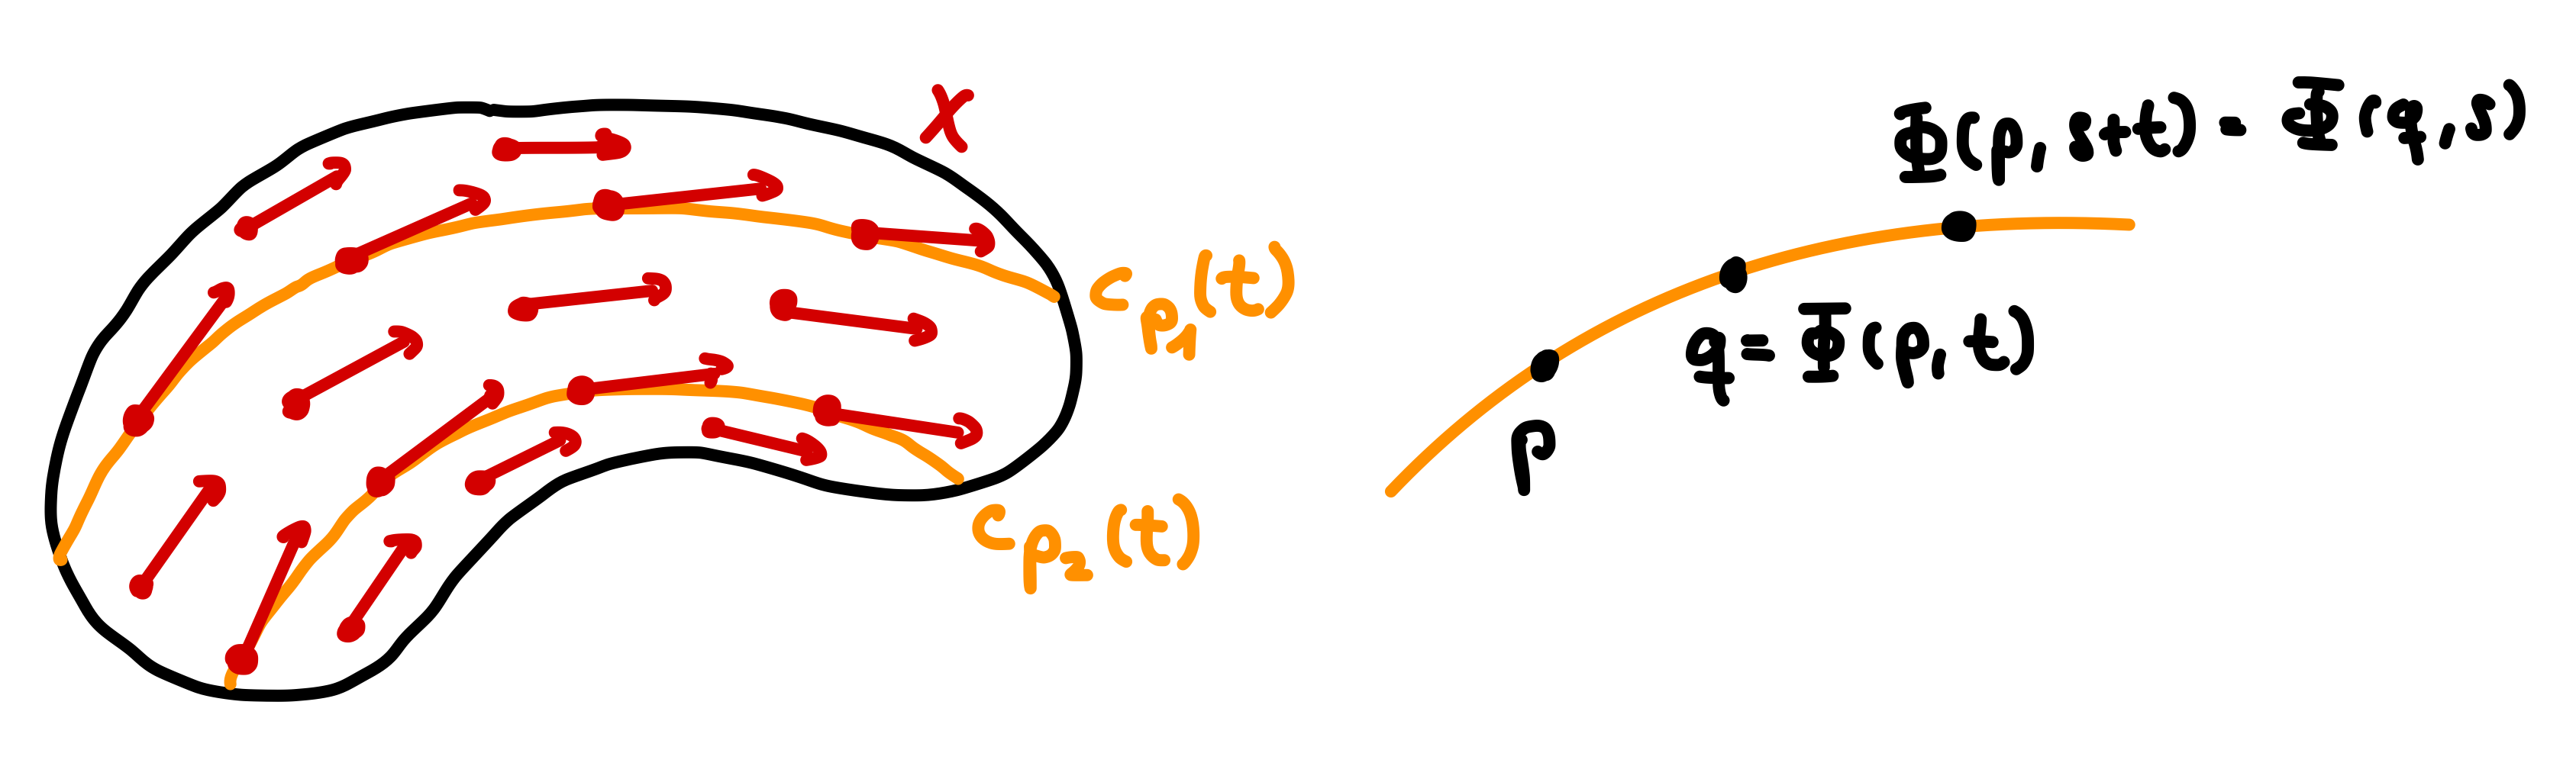
\includegraphics[width=0.5\linewidth]{Bilder/maxlsg.png}
\caption{Die Integralkurven auf einer MFK und die Funktion $\Phi$.}
\end{figure}
\end{satz}
\begin{beweis}
Die erste Bedingung folgt aus dem Satz von Picard-Lindelöf. Die zweite Bedingung folgt aus einem Satz über ODEs. Die letzte Bedingung ist ein Eindeutigkeitssatz.
\end{beweis}
\begin{definition}{Vollständigkeit}{vollst}
Ein Vektorfeld $X$ auf $M$ heißt \textbf{vollständig}, falls $\Ds_X = M \times \R$ gilt, also für jedes $p \in M$ die maximale Integralkurve durch $p$ für alle Zeiten $t \in \R$ definiert ist.
\end{definition}
\begin{bemerkungen}
\begin{enumerate}
\item Aus der lokalen Lösungstheorie erhält man, dass jedes Vektorfeld auf einer unberandeten, kompakten MFK vollständig ist.
\item Wir definieren den \textbf{Träger von} $X$ als $\supp X = \overline{\{ p \in M | X_p \neq 0 \}}$. Jedes Vektorfeld mit kompaktem Träger ist vollständig.
\begin{figure}[H]
\label{fig:kompaktesfeld}
\centering
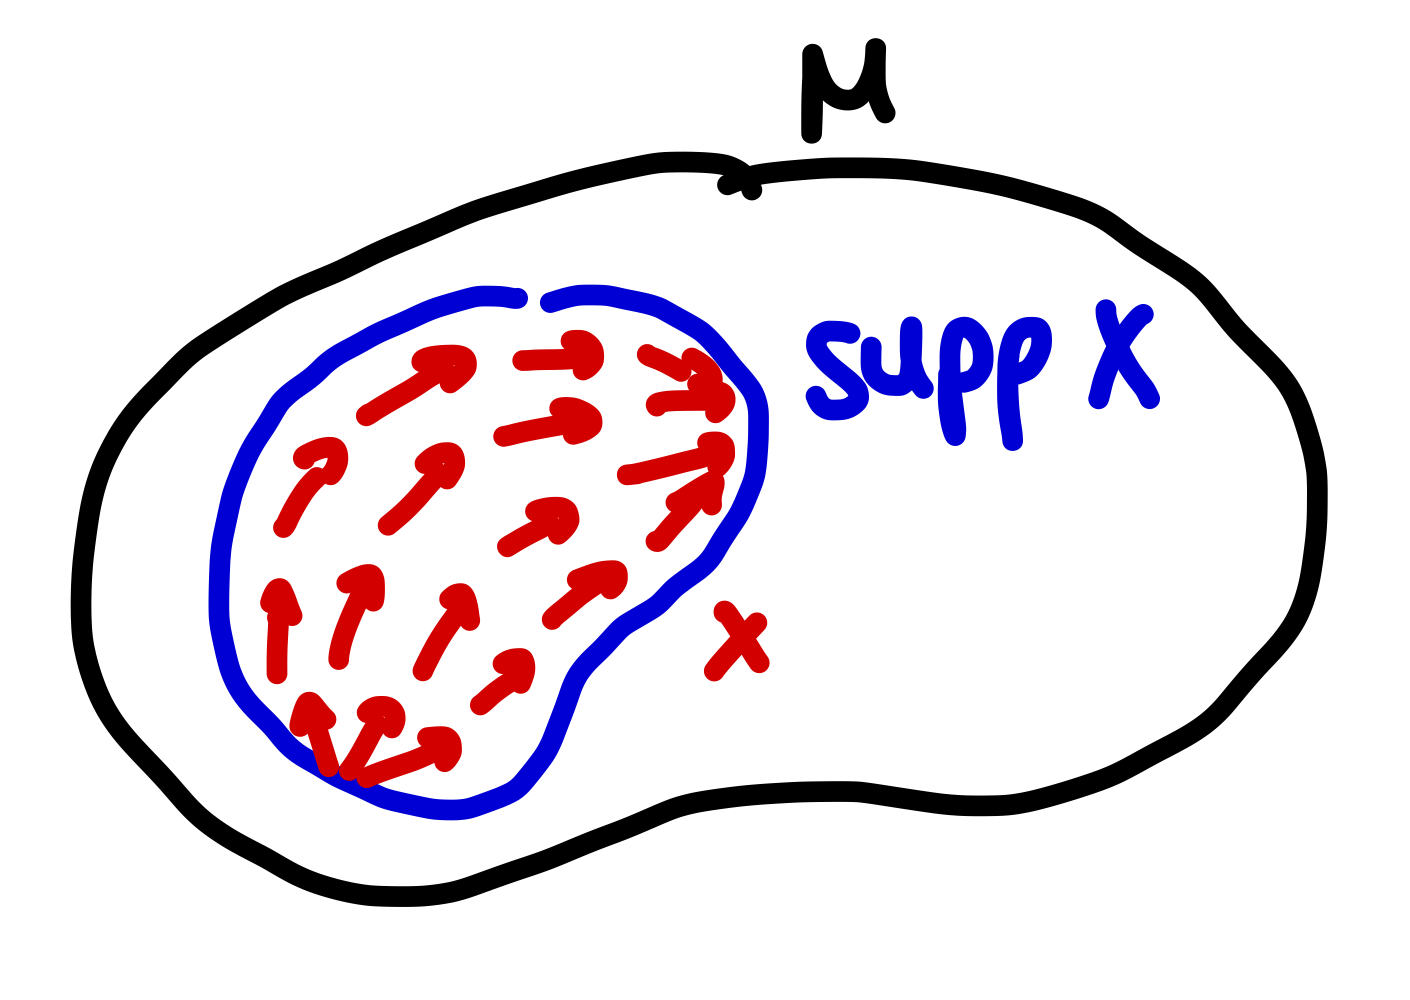
\includegraphics[width=0.2\linewidth]{Bilder/kmpktvektor.png}
\caption{Ein Vektorfeld mit kompaktem Träger.}
\end{figure}
\end{enumerate}
\end{bemerkungen}
\begin{beispiele}
\begin{enumerate}
\item Auf $M = \R^2$ betrachten wir das Vektorfeld
\begin{equation}
X_{(x,y)} := x \frac{\partial}{\partial y} - y \frac{\partial}{\partial x}.
\end{equation}
Dieses Vektorfeld ist vollständig mit
\begin{equation}
\Phi \left( \cvc{x,y}, t \right) = \mat{\cos t, - \sin t}{\sin t, \cos t}\cvc{x,y}.
\end{equation}
Entfernt man eine abgeschlossene Teilmenge $A \sub \R^2$ wie im Bild, so ist die Einschränkung von $X$ auf $\R^2 \times A$ nicht mehr vollständig.
\begin{figure}[H]
\label{fig:vektorfeldbsp}
\centering
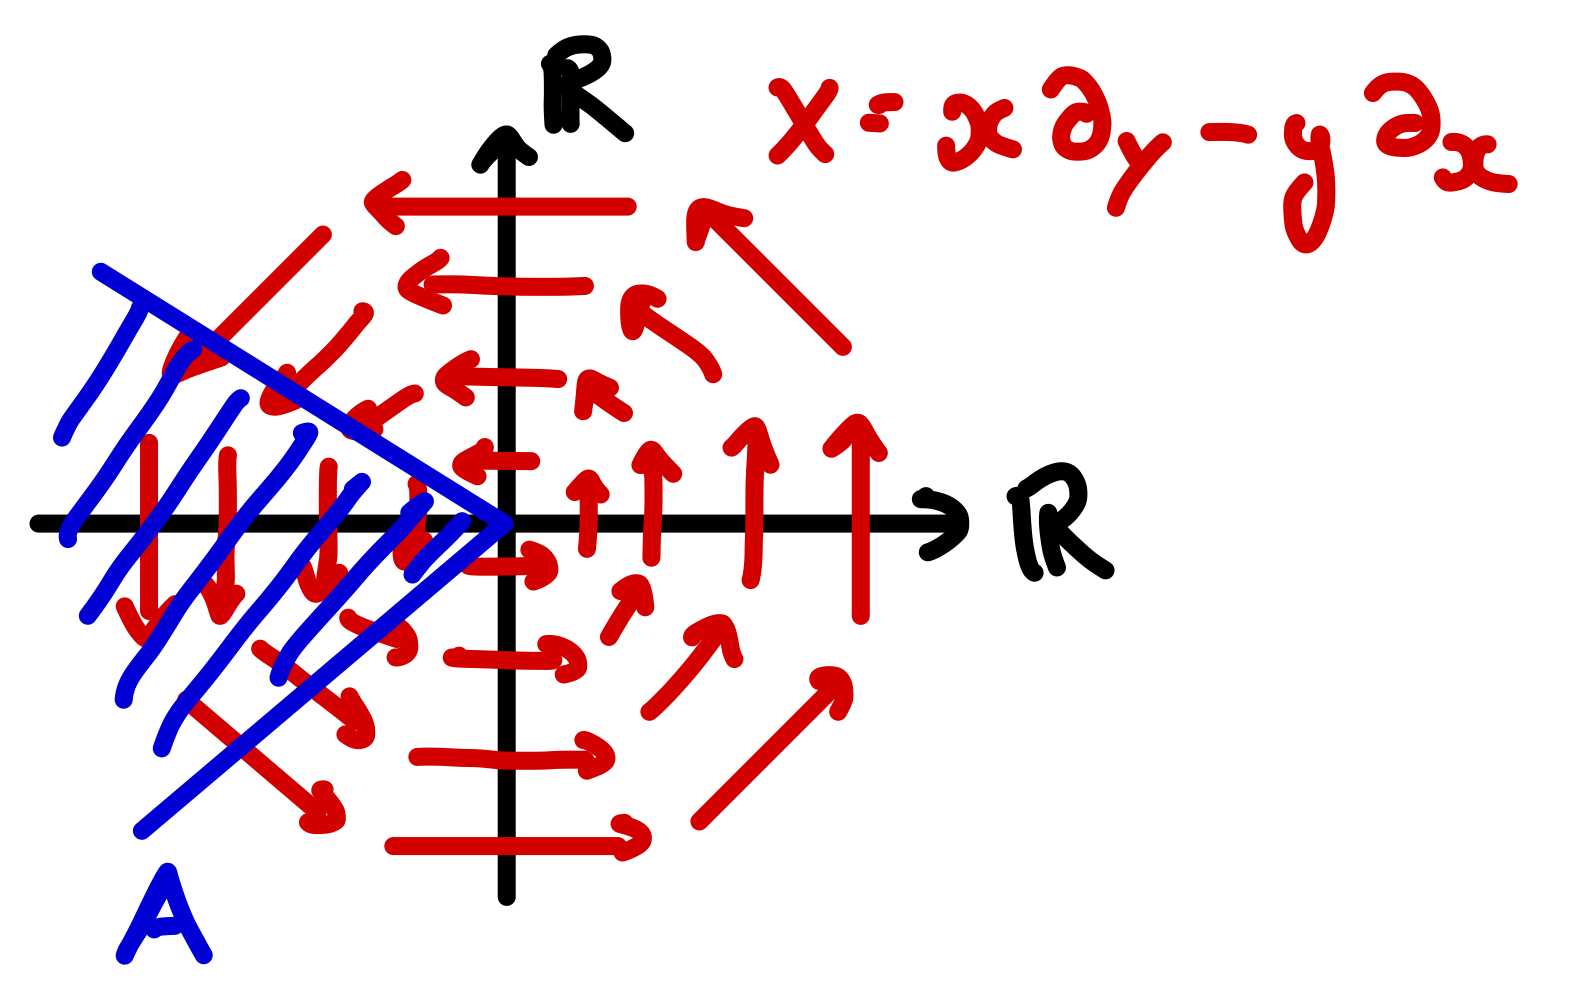
\includegraphics[width=0.2\linewidth]{Bilder/vektorfeldbsp.png}
\caption{Das Vektorfeld $X_{(x,y)}$ mit einer entnommenen Teilmenge $A \sub \R^2$.}
\end{figure}
\item Wir betrachten $M \sub \sph^2 \sub \R^3$ und wählen $v \in \sph^2$ fest. Wir definieren nun Vektorfelder $X$ und $Y$ auf $\sph^2$ als $X_p := v \times p$ und $Y_p := X_p \times p = (v \times p) \times p$.\footnote{$\times$ ist hier das Kreuzprodukt.} 
\end{enumerate}
\end{beispiele}
Hier ist es sinnvoll, den Einschub zur Lösungstheorie von ODEs anzuschauen.
\begin{satz}{Einparametergruppe von Diffeomorphismen}{einparameterdiff}
Sei $M$ eine glatte MFK und $X \in \Gamma(TM)$ vollständig, d.h. $I_p = \R$ für alle $p$. Die Abbildung
\begin{align}
\Phi: M \times \R &\to M \\
(p,t) &\mapsto c_p(t)
\end{align}
ist global definiert, wobei $c_p: I_p \to M$ die Integralkurve von $X$ mit $c_p(0)=p$ ist. Für $t \in \R$ fest erhalten wir:
\begin{align}
\phi_t: M &\to M \\
p &\mapsto \Phi(p,t).
\end{align}
Es gilt $\phi_0 =\id$ und $\phi_{t+s}=\phi_t\phi_s$. Insbesondere ist $\phi_t: M \to M$ invertierbar mit $(\phi_t)^{-1}=\phi_{-t}$.\\
Das bedeutet: Die Abbildung
\begin{align}
\R &\to \text{Diff}(M)\\
t &\mapsto \phi_t
\end{align}
ist ein \textit{Gruppenhomomorphismus}. Man nennt das Bild die zum Vektorfeld $X$ gehörende \textbf{Einparametergruppe} von Diffeomorphismen. $\phi_t$ heißt \textbf{Fluss} des Vektorfeldes $X$.
\begin{figure}[H]
\label{fig:fluss}
\centering
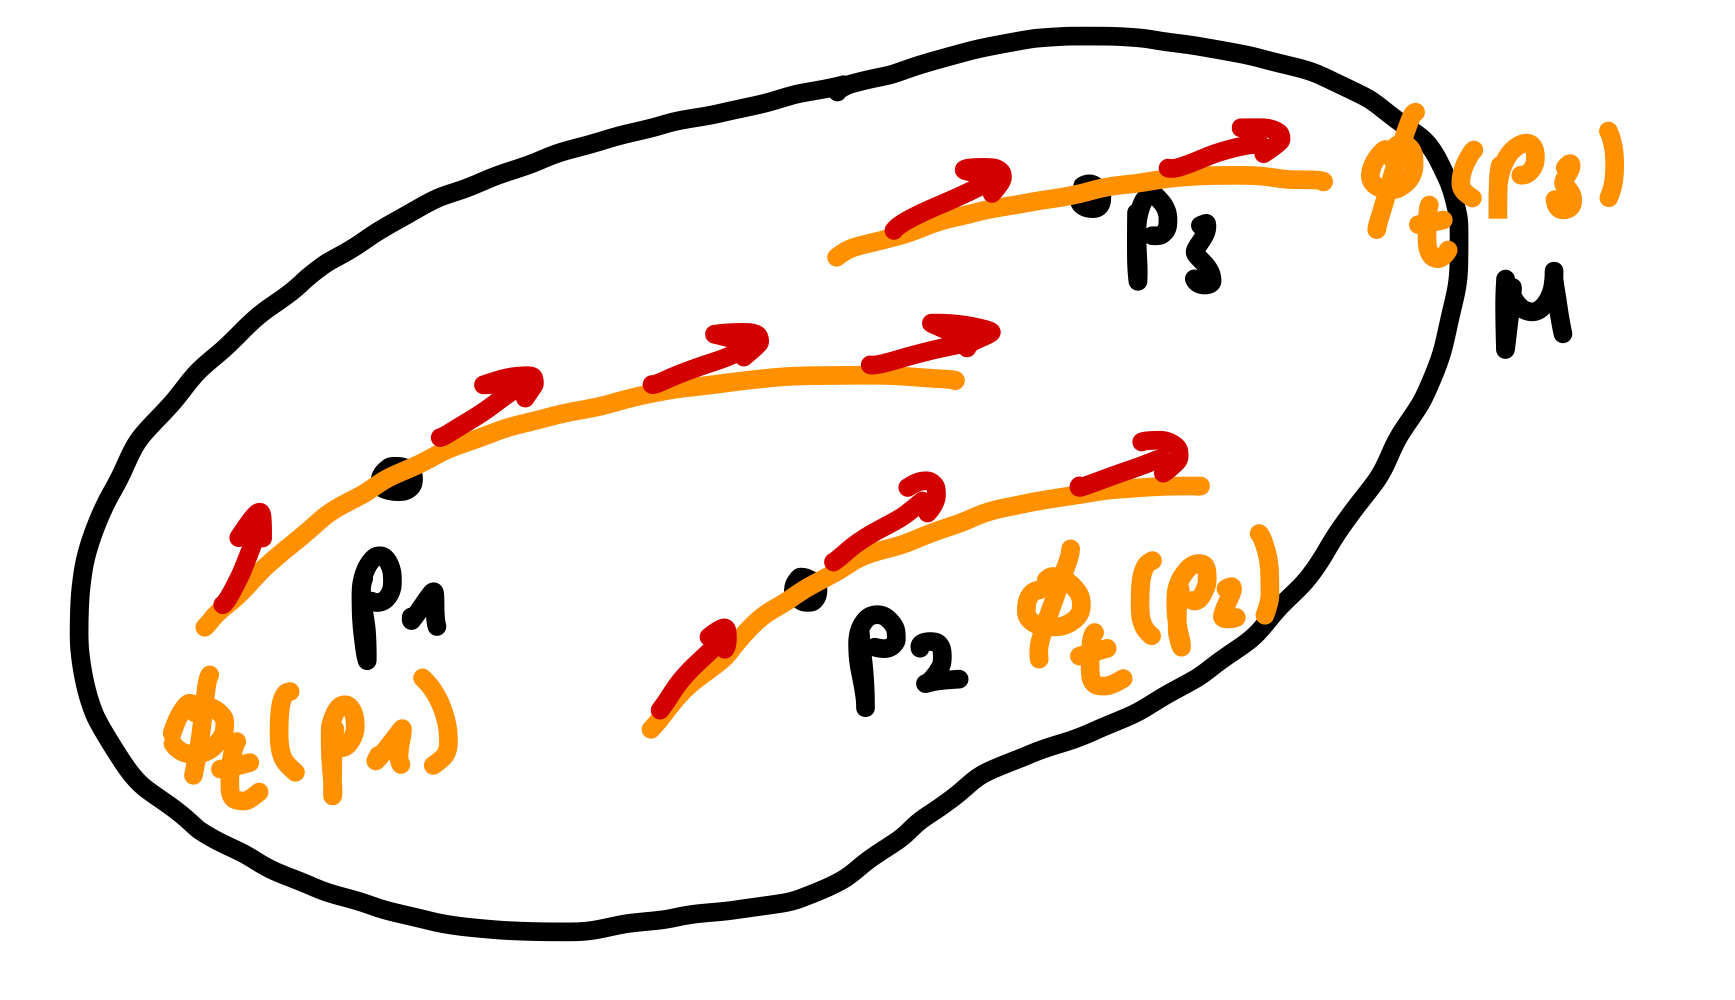
\includegraphics[width=0.25\linewidth]{Bilder/diffgruppe.png}
\caption{Die Diffeomorphismen ordnen jedem Punkt auf der MFK einen Punkt auf einer Integralkurve zu.}
\end{figure}
\end{satz}
\begin{bemerkung}
Ist umgekehrt $h: \R \to \text{Diff}(M)$ ein Gruppenhomomorphismus, sodass die Abbildung $\Psi: M \times \R \to M, \ (p, t) \mapsto h(t)(p)$ glatt ist, so kommt $h$ auch von einem Vektorfeld $X_p := \frac{d}{dt} \Psi(p,t)|_{t=0}$.
\end{bemerkung}
In der Definition von Ableitungen von Objekten im $\R^n$ wird sehr wesentlich die Vektorraumstruktur des $\R^n$ verwendet. Sei dazu z.B. $V: \R^n \to \R^n$ ein Vektorfeld. Wir wollen die Änderung von $V$ entlang einer Kurve $c: (a,b) \to \R^n$ verstehen. Dann bilden wir den Grenzwert
\begin{equation}
\lim_{t \to t_0} \frac{V(c(t))-V(c_0(t))}{t-t_0}.
\end{equation}
In einer MFK ist der entsprechende Ausdruck sinnlos, da $V(c(t)) \in T_{c(t)}M$ und $V(c(t_0)) \in T_{c(t_0)}M$ in \textit{verschiedenen Vektorräumen} liegen. Daher wollen wir den Fluss eines Vektorfeldes $X$ verwenden, um einen ersten sinnvollen Ableitungsbegriff auf MFKn zu definieren.
\begin{definition}{Lie-Ableitung}{lieabl}
Sei $M$ eine glatte MFK, $X, Y \in \Gamma(TM)$ und $\phi_t$ der Fluss von $X$.\\
Die \textbf{Lie-Ableitung von} $Y$ \textbf{in Richtung} $X$ ist das Vektorfeld $\Ls_XY \in \Gamma(TM)$, dessen Wert im Punkt $p \in M$ durch
\begin{equation}
(\Ls_XY)_p := \lim_{t \to 0} \frac{(\phi_{-t})_\ast Y_{\phi_t(p)} - Y_p}{t}
\end{equation}
gegeben ist.
\begin{figure}[H]
\label{fig:lieabl}
\centering
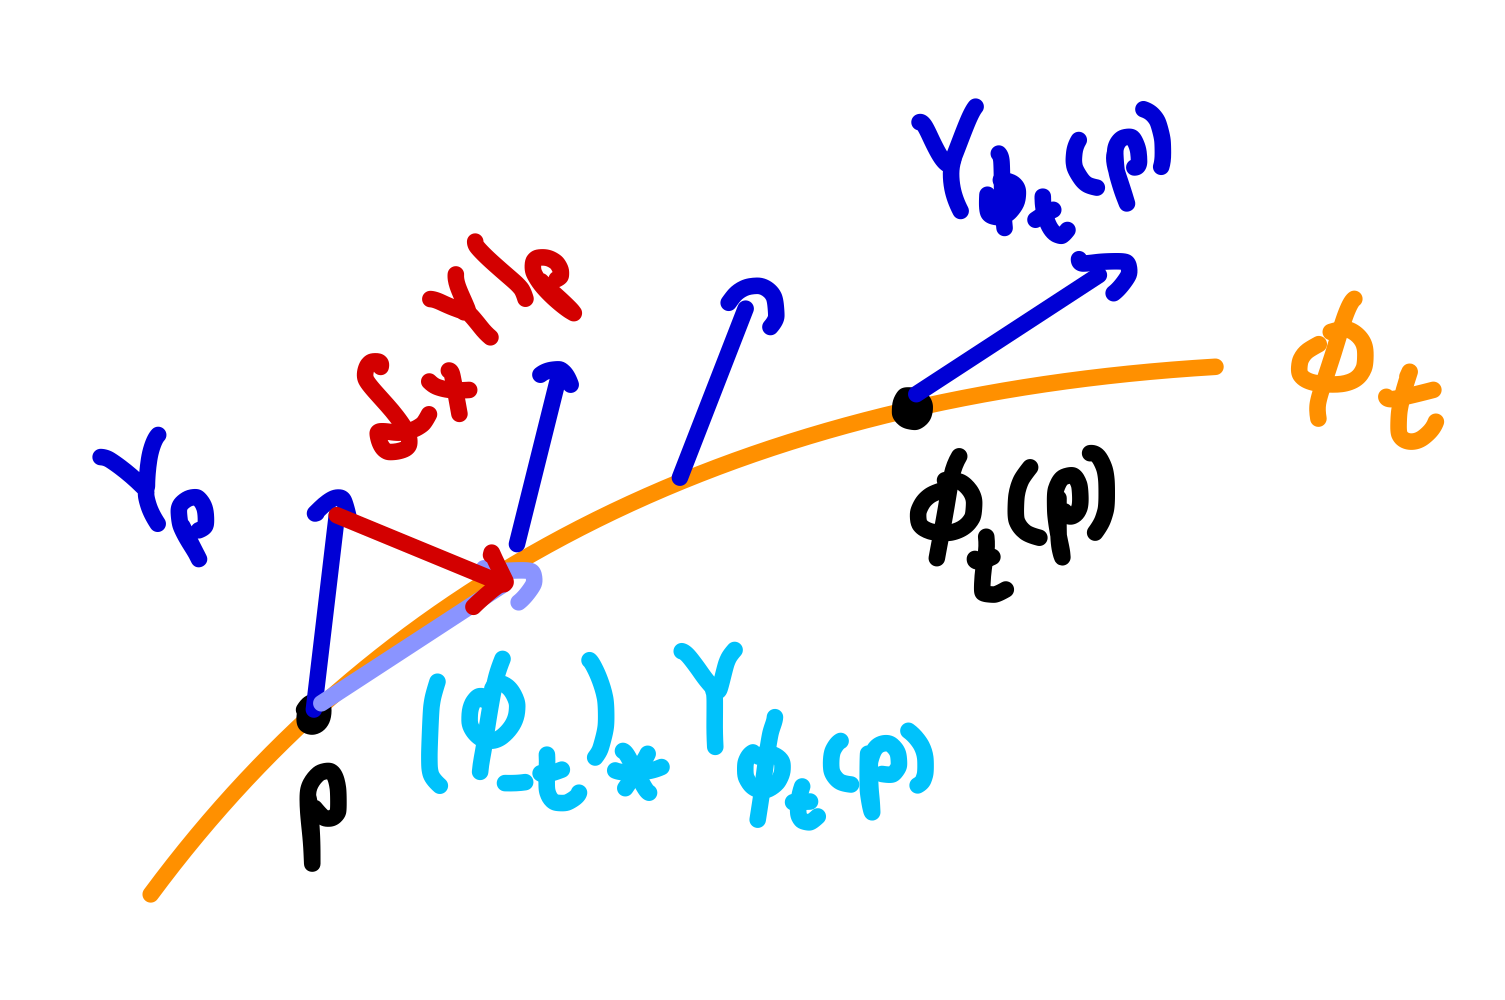
\includegraphics[width=0.4\linewidth]{Bilder/lieabl.png}
\caption{Die Lie-Ableitung eines Vektorfeldes $Y$ in Richtung $X$.}
\end{figure}
\end{definition}
\begin{bemerkung}
Wir wissen, dass $\phi_t \to^{t \to 0} \id_M$ und $\phi_{t\ast} \to^{t \to 0} \id_{TM}$. Deshalb können wir $\Ls_XY|_p$ auch schreiben als 
\begin{equation}
(\Ls_XY)_p = \lim_{t \to 0} \phi_{t\ast} \left( \frac{(\phi_{-t})_\ast Y_{\phi_t(p)} - Y_p}{t}\right) = \lim_{t\to 0} \frac{ Y_{\phi_t(p)} - (\phi_t)_\ast Y_p}{t} \in T_{\phi_t(p)}M.
\end{equation}
\end{bemerkung}
\begin{satz}{Lie-Klammer und Lie-Ableitung}{lieklammerableitung}
Es gilt $\Ls_X Y=[X, Y] (= - L_Y X)$.
\begin{figure}[H]
\label{fig:lieablklammer}
\centering
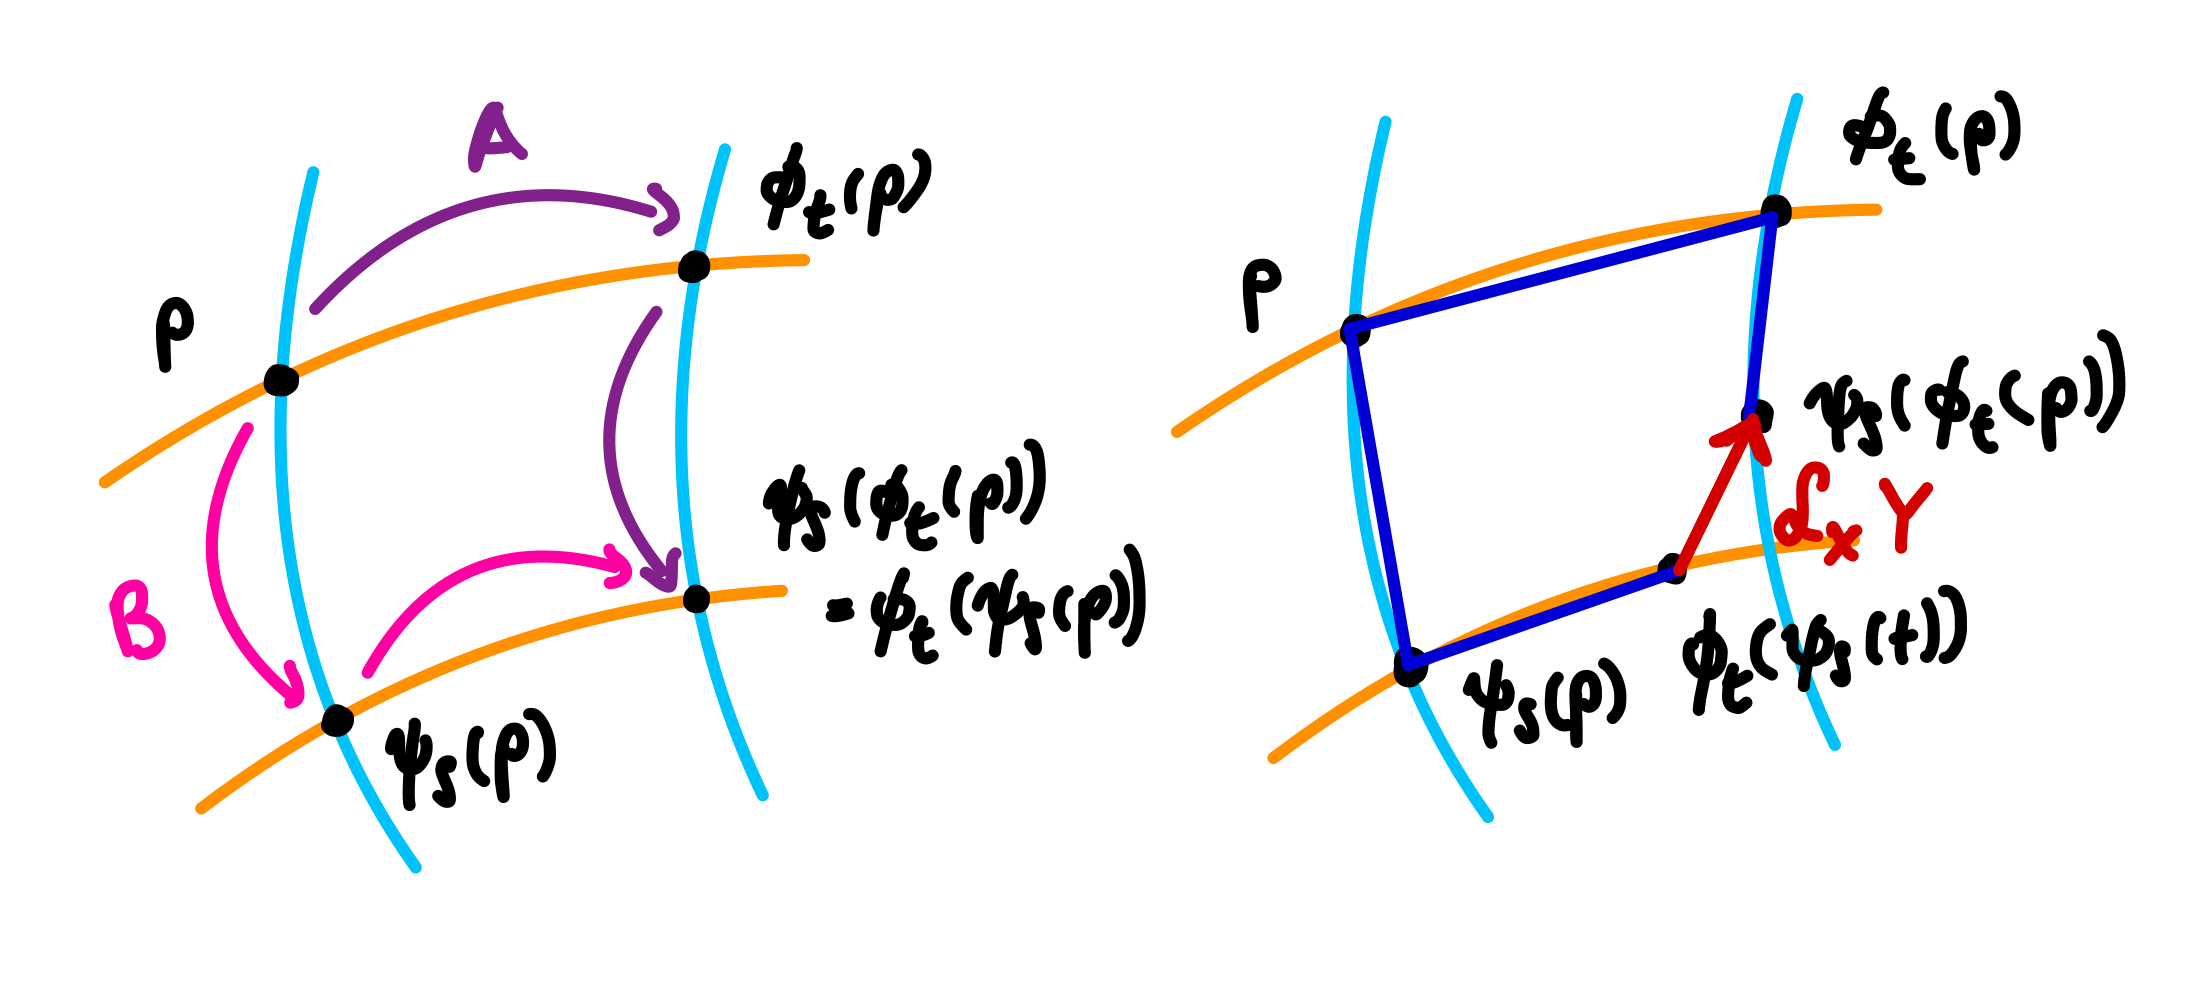
\includegraphics[width=0.4\linewidth]{Bilder/lieablklammer.png}
\caption{Links: Die Lie-Ableitung für Vektorfelder, deren Flüsse kommutieren, verschwindet. Rechts: Die Lie-Ableitung ''ergänzt'' das von den nicht-kommutierenden Flüssen aufgespannte Parallelogramm.}
\end{figure}
\end{satz}
\begin{beweis}
Wir führen den Beweis, indem wir die Wirkung beider Vektorfelder auf eine Funktion $f \in \cinf{M}$ vergleichen. Wir bezeichnen mit $\phi_t$ den Fluss von $X$ und mit $\psi_s$ den Fluss von $Y$. Nun definieren wir für $f\in \cinf{M}$ eine Funktion 
\begin{equation}
A(t):= Y_{\phi_t(p)}(f) = \frac{\partial}{\partial s} f(\psi_s(\phi_t(p)))|_{s=0}.
\end{equation}
und eine Funktion
\begin{equation}
B(t) := (\phi_t)_\ast Y_p(f) = Y_p(f \circ \phi_t) = \frac{\partial}{\partial s} f(\phi_t(\psi_s(p)))|_{s=0}.
\end{equation}
Dann gilt $A(0)=B(0)$ und außerdem 
\begin{align}
(L_XY)_p (f) &= \lim_{t \to 0} \frac{A(t)-B(t)}{t} = \lim_{t \to 0} \frac{A(t) - A(0)}{t} - \lim_{t \to 0} \frac{B(t)-B(0)}{t}\\
&= \frac{\partial^2}{\partial t \partial s} f(\psi_s \phi_t (p))|_{(s, t)=(0,0)} - \underbrace{\frac{\partial^2}{\partial t \partial s}}_{=\frac{\partial^2}{\partial s \partial t}} f(\phi_t \psi_s (p))|_{(s,t)=(0,0)} \\
&= X_p \left( \frac{\partial}{\partial s} (f \circ \psi_s(p))|_{s=0} \right) - Y_p \left( \frac{\partial}{\partial t} (f \circ \phi_t(p))|_{t=0}\right) = X_p(Y(f))- Y_p(X(f)) = [X, Y]_p (f)
\end{align}
\end{beweis}
\begin{korollar}{Aus \ref{lieklammerableitung}}{auslieklammerableitung}
Seien $X, Y \in \Gamma(TM)$ Vektorfelder mit Flüssen $\phi_t$ von $X$ und $\psi_s$ von $Y$. Gilt $[X, Y] =0$, so ist $\phi_t \psi_s = \psi_s \phi_t$ für alle $t,s$, sodass die Ausdrücke für alle $\tau \in [0,t]$ und alle $\sigma \in [0,s]$ definiert sind.
\end{korollar}
\begin{beweis}
$(\Rightarrow)$: Wir wissen, dass $[X,Y]_p(f)=\frac{\partial^2}{\partial t \partial s} f(\psi_s \phi_t (p)))|_{(s,t)=(0,0)} - \frac{\partial^2}{\partial t \partial s} f(\psi_t \phi_s (p)))|_{(s,t)=(0,0)} =0$, da die Flüsse nach Voraussetzung kommutieren.\\
$(\Leftarrow)$: Aus dem vorigen Satz wissen wir, dass 
\begin{equation}
[X, Y]_q = (L_XY)_q = \frac{d}{dt} ((\phi_{-t})_\ast Y_{\phi_t(q)})|_{t=0}.
\end{equation}
Für $t_0 \in I_q$ gilt dann
\begin{equation}
(\phi_{-t_0})_\ast [X,Y]_{\phi_{t_0}(q)} = (\phi_{-t_0})_\ast \left( \frac{d}{dt} (\phi_{-t})_\ast Y_{\phi_t(\phi_{t_0}(q)} \right)|_{t=0} = \frac{d}{d \tau} (\phi_{-\tau})_\ast Y_{\phi_\tau(q)})|_{\tau = t_0}.
\end{equation}
Wenn also $[X,Y]=0$ auf einer Umgebung von $p$, dann ist die Kurve $(-\epsilon, \epsilon) \to T_qM, \ t \mapsto (\phi_{-t})_\ast Y_{\phi_t(q)}$ für alle $q$ nahe $p$ konstant. Also gilt $Y_{\phi_t(q)} = (\phi_t)_\ast Y_q$ für $t$ nahe $0$ und $q$ nahe $p$. Wir betrachten nun die Kurven (für festes $t$) $\gamma_1 = \psi_s(\phi_t (p))$ und $\gamma_2 (s) = \phi_t (\psi_s (p))$. Es gilt: 
\begin{itemize}
\item $\gamma_1(0) = \gamma_2(0) = \phi_t(p)$
\item $\gamma_1$ erfüllt die DGL $\dot{\gamma}_1(s)=Y_{\gamma_1}(s)$.
\item $\gamma_2$ erfüllt diese DGL ebenfalls, denn 
\begin{equation}
\frac{d}{ds} \gamma_2(s) = (\phi_t)_\ast (\frac{d}{ds} \psi_s(p)) = (\phi_t)_\ast Y_{\psi_s(p)} = Y_{\phi_t\psi_s (p)} = Y_{\gamma_2(s)}.
\end{equation}
\end{itemize}
Aus der Eindeutigkeit der Lösung des AWP folgt $\gamma_1 (s) =  \gamma_2(s)$ für alle $s$.
\end{beweis}
\subsection{Liegruppen}
\label{subsec:liegruppen}
\begin{definition}{Lie-Gruppe}{liegruppe}
Eine \textbf{Lie-Gruppe} ist eine Gruppe $G$, sodass die zugrundeliegende Menge $G$ eine glatte MFK ist und die Strukturabbildungen 
\begin{align}
m: G \times G &\to G\\
g,h &\mapsto g \circ h
\end{align}
und
\begin{align}
i: G &\to G\\
g &\mapsto g^{-1}
\end{align}
glatte Abbildungen sind.
\end{definition}
\begin{beispiele}
\begin{enumerate}
\item $(\R^n, +)$: Auch Quotienten bezüglich einer diskreten Untergruppe, z.B. $\T^n = \quotient{\R^n}{\Z^n}$ sind Lie-Gruppen.
\item $\text{GL}(n, \R)$: Multiplikation und Inversenbildung sind glatt.
\item $\text{SL}(n, \R) := \{ A \in \text{GL}(n, \R) | \det (A) =1 \}$: $1$ ist ein regulärer Wert von $\det: \text{Mat}(n,\R) \to \R$, also ist $\text{SL}(n, \R)$ eine Untergruppe und UMF.
\item Mit demselben Argument:
\begin{itemize}
\item $\text{O}(n) := \{ A \in \text{GL}(n, \R) | A^TA = \id \}$.
\item $\text{SO}(n) := \text{O}(n) \cap \text{SL}(n, \R)$
\item $\text{U}(n) := \{ A \in \text{GL}(n, \C) | \bar{A}^TA=\id \} \sub \text{GL}(n, \C) \sub \text{GL}(2n, \R)$. Multiplikation mit $i$, aufgefasst als lineare Abbildung $\R^{2n} \to \R^{2n}$ hat bezüglich der Standardbasis $\R^n \oplus i \R^n$ die Form
\begin{equation}
J_0 = \mat{0, -\id}{\id, 0}.
\end{equation} 
Also gilt $\text{GL}(n, \C) = \{ A \in \text{GL}(2n, \R) | A J_0 = J_0 A\}$.
\item $\text{SU}(n) = \text{U}(n) \cap \text{SL}(2n, \R)$.
\end{itemize}
\item In kleineren Dimensionen trifft man alte Bekannte:
\begin{itemize}
\item $\text{SO}(2) \cong  \sph^1$
\item $\text{SO}(3) \cong \R P^3$ (als MFK)
\item $\text{SU}(2) \cong \sph^3$ (als MFK)
\end{itemize}
\end{enumerate}
\end{beispiele}
\begin{bemerkung}
In jeder Lie-Gruppe $G$ definiert jedes Element $h \in G$ zwei Diffeomorphismen:\\
Linksmultiplikation
\begin{align}
L_h: G &\to G \\
g &\mapsto hg
\end{align}
und Rechtsmultiplikation
\begin{align}
R_h: G &\to G\\
g &\mapsto gh.
\end{align}
Es gilt $R_h = L_h \iff h$ liegt im Zentrum von $G$, also $\forall h \in G: R_h = L_h \iff G$ kommutativ ist.
\end{bemerkung}
\begin{definition}{Linksinvarianz}{linksinvarianz}
Ein Vektorfeld $X \in \Gamma (TG)$ auf einer Lie-Gruppe $G$ heißt \textbf{linksinvariant}, falls $X_{hg} = X_{L_h(g)}=(L_h)_\ast X_g$ für alle $g,h \in G$.
\end{definition}
\begin{bemerkung}
Sei $e \in G$ das neutrale Element der Gruppe. Ist $X$ linksinvariant, so gilt $X_g = X_{L_g(e)} = (L_g)_\ast X_e$. Also sind linksinvariante Vektorfelder eindeutig bestimmt durch ihren Wert in $e \in G$. Umgekehrt definiert diese Formel für jedes $v = X_e \in T_eG$ ein linksinvariantes Vektorfeld, da 
\begin{equation}
X_{gh} = (L_{gh})_\ast X_e = (L_g)_\ast (L_h)_\ast X_e = (L_g)_\ast X_h
\end{equation}
für alle $g, h \in G$ gilt. Also sind linksinvariante Vektorfelder in Bijektion zu $T_eG$.
\end{bemerkung}
\begin{beispiel}
Auf $(\R^n, +)$ sind linksinvariante Vektorfelder translationsinvariante Vektorfelder, d.h. sie haben als Linearkombination der Koordinatenvektorfelder $\frac{\partial}{\partial x_1}, \dots, \frac{\partial}{\partial x_n}$ konstante Koeffizienten.
\end{beispiel}
\begin{lemma}{Linksinvarianz der Lie-Klammer}{linksinvariantelieklammer}
Für linksinvariante Vektorfelder $X,Y$ ist auch $[X, Y]$ linksinvariant.
\end{lemma}
\begin{beweis}
Gemäß Übung (A12) gilt: 
\begin{equation}
[X,Y] = [(L_h)_\ast X, (L_h)_\ast Y]= (L_h)_\ast [X,Y]
\end{equation}
für alle $h \in G$.
\end{beweis}
\begin{korollar}{Lie-Unteralgebra der VF}{lieunteralgebra}
Die linksinvarianten Vektorfelder bilden eine Lie-Unteralgebra in $\Gamma (TG)$.
\end{korollar}
\begin{beweis}
Umformulierung des vorigen Lemmas.
\end{beweis}
\begin{bemerkung}
Indem wir die Identifikation der linksinvarianten Vektorfelder mit dem Tangentialraum $\mathfrak{g}:= T_eG$ vornehmen, erhalten wir eine Lie-Algebra-Struktur:
\begin{align}
[.,.]: \mathfrak{g} \times \mathfrak{g} &\to \mathfrak{g}\\
(\xi, \eta) &\mapsto [X, Y]_e,
\end{align}
wobei $X$ und $Y$ die linksinvarianten Fortsetzungen von $\xi$ und $\eta$ sind.
\end{bemerkung}
\begin{beispiele}
\begin{enumerate}
\item Für $G=(\R^n,+)$ ist die Lie-Klammer auf $\mathfrak{g} \cong \R^n$ trivial, also $[u,v]=0$ für alle $u, v \in \R^n$.
\item Für $G = \text{GL}(n, \R)$ ist $\mathfrak{gl}(n, \R) = \text{Mat}(n, \R)$.
\end{enumerate}
\end{beispiele}
\begin{satz}{Lie-Klammer auf $\mathfrak{gl}(n,\R)$}{lieklammergl}
Die Lie-Klammer auf $\mathfrak{gl}(n, \R)$ hat die Form $[\xi, \eta] = \xi \eta - \eta \xi$.
\end{satz}
\begin{beweis}
Für festes $h \in \text{GL}(n, \R)$ ist die Linksmultiplikation 
\begin{align}
L_h: \text{GL}(n, \R) &\to \text{GL}(n, \R)\\
g &\mapsto hg
\end{align}
linear in $g$, sodass
\begin{equation}
(L_h)_\ast = L_h: \text{Mat}(n,\R) \to \text{Mat}(n, \R).
\end{equation}
Also ist für $\xi \in T_\id \text{GL}(n, \R)$ das zugehörige linksinvariante Vektorfeld $X$, gegeben als $X_g = g \cdot \xi$. Die Gleichung $\dot{g}(t) = X_{g(t)} = \xi g(t)$ hat die eindeutige Lösung $g(t) = g(0) \exp (t \xi)$. Der Fluss $\phi_t$ von $X$ hat also die Form $\phi_t (g) = g \exp (t \xi)$. Wie zuvor gilt $(\phi_t)_\ast = R_{\exp (t \xi)}$. Sind nun $\xi, \eta \in T_\id \text{GL}(n, \R)$ mit zugehörigen linksinvarianten Vektorfeldern $X$ und $Y$, so gilt
\begin{equation}
[\xi, \eta] = [X,Y]_\id = (\Ls_XY)_\id = \left.\frac{d}{dt} \left( (\phi_t)_\ast Y_{\phi_t(\id)} \right)\right|_{t=0}=\left. \frac{d}{dt} \exp(t \xi) \eta \exp(-t \xi) \right|_{t=0} = \xi \eta- \eta \xi.
\end{equation}
\end{beweis}
\begin{figure}[H]
\label{fig:linksinvariant}
\centering
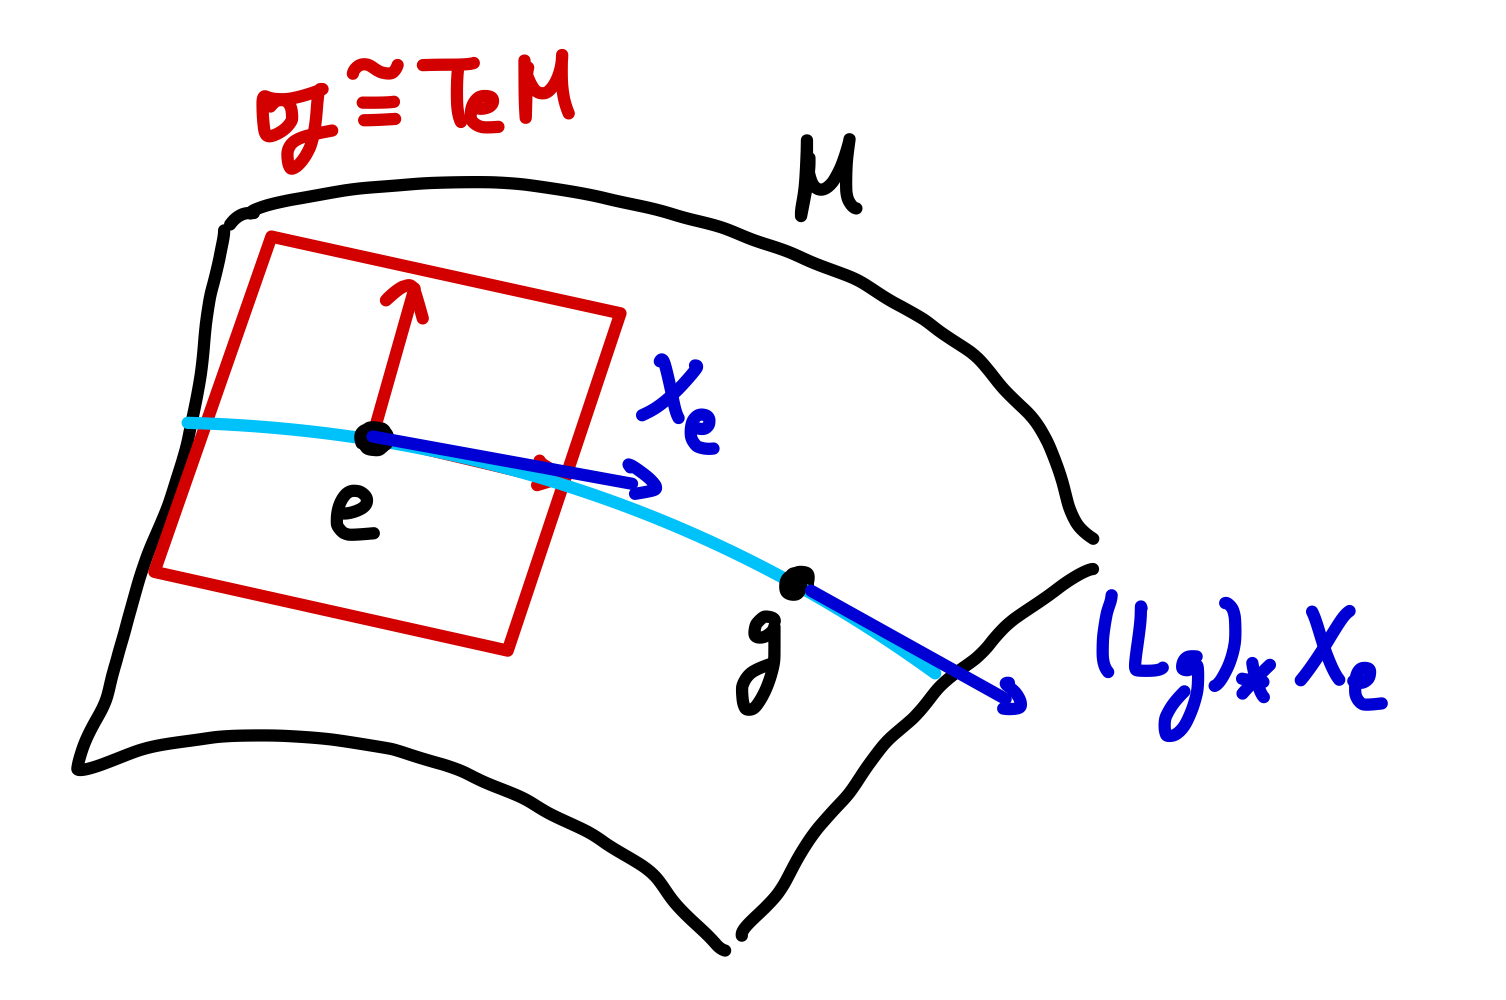
\includegraphics[width=0.3\linewidth]{Bilder/linksinvariant.png}
\caption{Eine Lie-Gruppe als Tangentialraum an der Identität mit linksinvariantem Vektorfeld.}
\end{figure}
\begin{bemerkung}
Die Rechnung zeigt: Linksinvariante Vektorfelder auf $\text{GL}(n, \R)$ sind vollständig. Das gilt allgemein für alle Lie-Gruppen: Ist $X \in \Gamma (TG)$ linksinvariant und $\gamma: I_e \to G$ die maximale Integralkurve durch $e \in G$, dann ist $L_g \circ \gamma: I_e \to G$ eine Integralkurve durch $g$
\begin{equation}
\frac{d}{dt}(L_g \circ \gamma) = (L_g)_\ast \dot{\gamma} = (L_g)_\ast X = X.
\end{equation}
Für $g = \gamma(t)$ mit $t \neq 0$ wissen wir, dass $I_g = I_e -t$, also geht $I_e \sub I_g$ für alle $g = \gamma (t)$ nur für $I_e = \R$.
\end{bemerkung}
\begin{definition}{Exponentialabbildung}{expabb}
Sei $G$ eine Lie-Gruppe. Die \textbf{Exponentialabbildung}
\begin{equation}
\exp: T_eG = \mathfrak{g} \to G
\end{equation}
ist definiert als $\exp (\xi) = \gamma_\xi (1)$, wobei $\gamma_\xi: \R \to G$ die Integralkurve des zu $\xi$ gehörenden, linksinvarianten Vektorfeldes mit $\gamma_\xi (0)=e$ ist.
\end{definition}
\begin{bemerkung}
Der Name Exponentialabbildung kommt daher, dass für Matrixgruppen $\exp(\xi) = e^\xi$ gilt.
\end{bemerkung}
\begin{beispiel}
Für $G = \quotient{\R^n}{\Z^n} \cong T^n$ ist die Exponentialabbildung $exp: \R^n \to \quotient{\R^n}{\Z^n}$ die universelle Überlagerung von $T^n$, d.h. die Abbildung, die $x\in \R^n$ auf seine Äquivalenzklasse $[x] \in T^n$ abbildet.
\end{beispiel}
\begin{satz}{Differential als Gruppenhomomorphismus}{diffhomo}
Ist $\phi: G \to H$ ein glatter Gruppenhomomorphismus, dann ist $\phi_{\ast, e}: \mathfrak{g} \to \mathfrak{h}$ ein Homomorphismus von Lie-Algebren.
\end{satz}
\begin{beweis}
Wir müssen zeigen, dass $\phi_\ast [\xi, \eta] = [\phi_\ast \xi, \phi_\ast \eta]$.\\
Dafür wollen wir ÜA (A12) nutzen. Um das dort gezeigte Ergebnis anwenden zu können, müssen wir zeigen, dass für die linksinvarianten Vektorfelder $X,Y$ auf $G$ zu $\xi, \eta$ bzw. $\overline{X}, \overline{Y}$ auf $H$ zu $\phi_\ast \xi, \phi_\ast \eta$ die Gleichung $\phi_\ast (X_g) = \overline{X}_{\phi(g)}$ und analog für $\overline{X}, \overline{Y}$ gilt.\\
$\phi$ ist ein Gruppenhomomorphismus, sodass gilt:
\begin{align}
\phi(gh) &= \phi(g) \phi(h) \\
\phi \circ L_g &= L_{\phi(g)} \phi \\
\implies \phi_\ast L_{g_\ast} &= L_{\phi (g)\ast} \phi_\ast\\
\iff \phi_\ast &= L_{\phi (g), \ast} \phi_\ast \underbrace{(L_{g \ast})^{-1}}_{(L_{g^{-1}})_\ast}.
\end{align}
Daraus folgt, dass
\begin{align}
\phi_\ast X_g &= L_{\phi(g)\ast} \phi_\ast (L_{g^{-1}})_\ast X_g\\
&= L_{\phi(g)\ast} \phi_\ast \xi \\
&= \overline{X}_{\phi(g)},
\end{align}
was zu zeigen war.
\end{beweis}
\begin{beispiel}
Wir betrachten den Gruppenhomomorphismus 
\begin{equation}
\det: GL(n, \R) \to \R^\ast = (\R \exc \{0\}, \cdot).
\end{equation}
Wir zeigen, dass $det_{\ast, \id} = \Tr: \text{Mat}(n, \R) \to \R$ gilt.\\
Seien $A \in \text{GL}(n, \R)$ und $\xi \in \text{Mat}(n, \R)$ mit Spaltenvektoren $a_1, \dots, a_n$ und $\xi_1, \dots, \xi_n$. Dann gilt 
\begin{equation}
\frac{d}{dt} \det (A+t \xi)|_{t=0} = \Sum{i,1,n} \det (a_1, \dots, a_{i-1}, \xi_i, a_{i+1}, \dots, a_n).
\end{equation}
Für $A = \id \in \text{GL}(n, \R)$ gilt dann
\begin{align}
\frac{d}{dt} \det (\id + t \xi)|_{t=0} &= (\det)_{\ast, \id}(\xi) \\
&= \Sum{i,1,n} \det \mat{1, 0, \cdots,0, \xi_{1i}, 0,0, \cdots, 0}{0, 1, \cdots,0, \xi_{2i}, 0,0, \cdots, 0}{\vdots, \vdots,  \ddots,\vdots, \vdots, \vdots,\vdots, \ddots, \vdots}{0,0,\cdots,1,\xi_{(l-1)i},0,0,\cdots,0}{0, 0, \cdots,0, \xi_{li}, 1,0, \cdots, 0}{0, 0, \cdots,0, \xi_{(l+1)i}, 0,1, \cdots, 0}{\vdots,\vdots, \ddots,\vdots, \vdots, \vdots, \vdots, \ddots, 0}{0,0, \cdots, 0, \xi_{ni}, 0,0,\cdots,1}\\
&= \Sum{i,1,n} \xi_{ii} = \Tr \xi.
\end{align}
\end{beispiel}
Auf $\R$ verschwindet die Lie-Klammer. Auf $\text{Mat}(n, \R)=\mathfrak{gl}(n, \R)$ gilt aber $[\xi, \eta] = \xi \eta - \eta \xi$. Der Satz sagt dann $\Tr(\xi \eta - \eta \xi)=\Tr (\xi \eta) - \Tr (\eta \xi)=0$. Wir erhalten also die bekannte Aussage $\Tr (\xi \eta) = \Tr (\eta \xi)$ für alle $\xi, \eta \in \mathfrak{gl}(n, \R)$.
\begin{bemerkungen}
Zwei wichtige Sätze von \emph{Lie} sagen:
\begin{enumerate}
\item Zu jeder endlich-dimensionalen Lie-Algebra $\mathfrak{g}$ existiert eine bis auf Isomorphie eindeutige, einfach-zusammenhängende Lie-Gruppe $G$ mit $T_eG=\mathfrak{g}$.
\item Ist $\overline{\phi}: \mathfrak{g} \to \mathfrak{h}$ eine Homomorphismus zwischen endlich-dimensionalen Lie-Algebren, so existiert für \textit{jede} Lie-Gruppe $H$ mit Lie-Algebra $\mathfrak{h}$ ein Gruppenhomomorphismus $\phi: G \to H$ von der einfach-zusammenhängenden Lie-Gruppe $G$ mit Lie-Algebra $\mathfrak{g}$ mit $\phi_{\ast, e} = \overline{\phi}$.
\end{enumerate}
\end{bemerkungen}
\begin{beispiel}
Hat die Lie-Algebra $\mathfrak{h}$ der Lie-Gruppe $H$ eine abelsche Lie-Unteralgebra $\mathfrak{h}_0 \sub \mathfrak{h}$, dann existiert eine abelsche Lie-Untergruppe $H_0 \sub H$ mit $T_eH_0 = \mathfrak{h}$.
\end{beispiel}
\subsection{Differentialformen auf Mannigfaltigkeiten}
\label{subsec:diffformen}
Die Theorie funktioniert ganz analog zum Fall von UMF des $\R^n$.
\begin{satz}{1-Formen als lokaler Rahmen}{formenlokrahmen}
Sei $Q$ eine glatte MFK, $TQ$ das Tangentialbündel und $T^\ast Q$ das Kotangentialbündel. Sind $(q_1, \dots, q_n)$ lokale Koordinaten auf $U \sub Q$, so sind die $1$-Formen $dq_1, \dots, dq_n$ ein lokaler Rahmen für $T^\ast Q|_M$.
\end{satz}
Jeder Punkt in $T^\ast Q|_M$ lässt sich also schreiben als $(q, \alpha_q)$ mit $q \in U$ und $\alpha_q \in T^\ast_q Q = \text{L}(T_q Q, \R)$. Dabei hat $\alpha_q$ eine eindeutige Darstellung als $\alpha_q = \Sum{j,1,n} p_j (d_{q_j})_q$ mit $p_j \in \R$.
\begin{bemerkung}Kanonische Koordinaten\\
$(q_1, \dots, q_n, p_1, \dots, p_n)$ bilden lokale Koordinaten auf $T^\ast Q|_U$. Man nennt diese Koordinaten auch die \textbf{kanonischen Koordinaten} auf $T^\ast Q|_U$ assoziiert zu den Koordinaten $(q_1, \dots, q_n)$ auf $U$.
\end{bemerkung}
\begin{satz}{Globale $1$-Form}{globdiff}
Durch $\lambda := \Sum{j,1,n} p_j dq_j$ wird eine $1$-Form auf $T^\ast Q|_U$ definiert. Diese in lokalen, kanonischen Koordinaten definierten $1$-Formen auf $T^\ast Q$ passen zusammen zu einer global definierten $1$-Form $\lambda_{\text{can}}$ auf $M = T^\ast Q$. Eine beliebige glatte $1$-Form $\alpha \in \Omega^1(Q)$ ist ein Schnitt in $T^\ast Q$, also eine Abbildung 
\begin{equation}
\alpha: Q \to T^\ast Q
\end{equation}
mit $\pi_\alpha = \id$.
\end{satz}
\begin{satz}{Pullback einer Differentialform}{pullbackdiff}
Für alle $\alpha \in \Omega^1 (Q)$ gilt $\alpha^\ast (\lambda_{\text{can}}) = \alpha$.
\end{satz}
\begin{bemerkung}
Es gilt $d\lambda_\text{can} \in \Omega^2(T^\ast Q)$. In lokalen, kanonischen Koordinaten gilt
\begin{equation}
d \lambda_\text{can} = \Sum{j,1,n} dp_j \wedge dq_j.
\end{equation}
Diese Form ist nicht-ausgeartet in dem Sinn, dass $T(T^\ast Q) \to T_x^\ast(T^\ast Q), \ v \mapsto i_v d \lambda_\text{can}$ ein Isomorphismus ist.\\
$(T^\ast Q, d \lambda_\text{can})$ ist ein Beispiel für eine \textit{symplektische MFK}.
\end{bemerkung}
\begin{definition}{Symplektische MFK}{symplek}
Ein Paar $(M, \omega)$ heißt \textbf{symplektische MFK}, wenn $\omega \in \Omega^2 (M)$ und $d\omega = 0$ gilt und $\omega$ nicht ausgeartet ist, d.h., dass $\forall p \in M$ 
\begin{align}
T_pM &\to T_p^\ast M \\
v &\mapsto \omega(v, .)
\end{align}
ein Isomorphismus ist.
\end{definition}
\begin{definition}{\textit{Hamiltonsches Vektorfeld}}{hamilton}
Sei $H: T^\ast \R^n \to \R$ eine glatte Funktion und $\omega = \omega_\text{can} \in \Omega^2(T^\ast \R^n)$ die kanonische symplektische Form. Dann definiert die Gleichung
\begin{equation}
X \iprod \omega = -dH
\end{equation}
das zu $H$ gehörige \textbf{Hamiltonsche Vektorfeld}.
\end{definition}
\begin{satz}{Invarianz unter $X$}{invarianz}
Sei $X$ das Hamiltonsche Vektorfeld der glatten Abbildung $H: T^\ast \R^n \to \R$ und $\omega_\text{can}$ die kanonische symplektische Form. Dann gilt für den Fluss $\phi_t: T^\ast \R^n \to \T^\ast \R^n$, dass 
\begin{equation}
\phi_t^\ast \omega = \omega,
\end{equation}
also ist $\omega$ invariant unter dem Fluss von $X$. Insbesondere ist die Volumenform $\mu:= \omega^{\wedge n} \in \Omega^{2n}(T^\ast \R^n)$ invariant unter $\phi_t$.
\end{satz}
\begin{beweis}
Übung 6.3
\end{beweis}
\begin{definition}{$k$-Formen}{kforms}
Glatte $k$\textbf{-Formen} auf $Q$ sind Schnitte in einem Bündel $\Lambda^k T^\ast Q \to Q$.
\end{definition}
Sind $q_1, \dots, q_n$ lokale Koordinaten auf $Q$, so bilden die Formen
\begin{equation}
dq^I := dq_{i_1} \wedge \cdots \wedge dq_{i_k}
\end{equation}
mit $\{ i_1 < \cdots < i_k \} =: I$ einen lokalen Rahmen für $\Lambda^k T^\ast Q$, d.h. jede glatte $k$-Form kann lokal geschrieben werden als
\begin{equation}
\eta|_U = \sum_{I = \{i_1 < \cdots  < i_k \}} \eta_I dq^I
\end{equation}
mit $\eta_I \in \cinf{U}$.
\begin{definition}{Äußeres Differential}{outerdiff}
Das \textbf{äußere Differential} $d: \Omega^k (Q) \to \Omega^{k+1} (Q)$ ist charakterisiert durch folgende Eigenschaften:
\begin{itemize}
\item Für Funktionen $f: Q \to \R$ gilt $df = f^\ast dt$, wobei $dt$ die Standard-$1$-Form auf $\R$ ist. Insbesondere gilt dann $df(X) = X(f)$.
\item $d(\eta_1 \wedge \eta_2) = (d \eta_1) \wedge \eta_2 + (-1)^{\text{deg} \ \eta_1} \eta_1 \wedge d \eta_2$.
\item $d^2 = 0$.
\end{itemize}
\end{definition}
\begin{definition}{\textit{Lie-Ableitung für Differentialformen}}{liedifferential}
Sei $M$ eine glatte MFK, $X \in \Gamma(TM)$ ein glattes Vektorfeld und $\omega \in \Omega^k(M)$ eine $k$-Form. Dann definiert
\begin{equation}
\Ls_x \omega := \lim_{t \to 0} \frac{\phi_t^\ast \omega - \omega}{t}
\end{equation}
die \textbf{Lie-Ableitungen für Differentialformen}, wobei $\phi_t$ der Fluss von $X$ ist.
\end{definition}
\begin{definition}{\textit{Inneres Produkt}}{inneresdifferential}
Sei $M$ eine glatte MFK und $X \in \Gamma(TM)$ ein glattes Vektorfeld. Dann ist das \textbf{innere Produkt} die lineare Abbildung
\begin{align}
\iprod: \Omega^k(M) &\to \Omega^{k-1}(M)\\
\omega &\mapsto X \iprod \omega(X_1, \dots, X_{k-1}) = \omega(X, X_1, \dots, X_{k-1}.
\end{align}
Man schreibt auch $X \iprod \omega = i_X \omega$.
\end{definition}
\begin{bemerkung}
Es gelten meherere Formeln für das innere Produkt, die in (A15) und (A16) bewiesen werden:
\begin{itemize}
\item Für alle $X \in \Gamma(TM)$ glatt, $\omega_1 \in \Omega^k(M)$ und $\omega_2 \in \Omega^l(M)$ gilt 
\begin{equation}
X \iprod (\omega_1 \wedge \omega_2) = (X \iprod \omega_1) \wedge \omega_2 + (-1)^k \omega_1 \wedge (X \iprod \omega_2).
\end{equation}
\item Sei $\eta \in \Omega^1(M)$ und $X,Y \in \Gamma(TM)$ glatt. Dann gilt
\begin{equation}
d\eta(X,Y) = X(\eta(Y))-Y(\eta(X))-\eta([X,Y]).
\end{equation}
\end{itemize}
\end{bemerkung}
\begin{theorem}{\textit{Cartans magische Formel}}{cartansmagie}
Sei $M$ eine glatte MFK, $X \in \Gamma(TM)$ glatt und $\omega \in \Omega^k(M)$ eine glatte $k$-Form. Dann gilt
\begin{equation}
\Ls_X \omega = d(X \iprod \omega) + X \iprod d\omega.
\end{equation}
\end{theorem}
Um über Integration zu reden, benötigen wir Orientierungen:
\begin{definition}{Orientierbarkeit}{orientierung}
$Q$ heißt \textbf{orientierbar}, falls es einen Atlas $\mathfrak{A} = \{ (U_\alpha, \phi_\alpha) \}_{\alpha \in I}$ gibt, sodass alle Übergangsabbildungen $\phi_{\alpha \beta}$ orientierungserhaltende Diffeomorphismen von offenen Teilmengen des $\R^n$ sind, d.h. die Ableitungen $\Ds \phi_{\alpha \beta}$ haben überall positive Determinante.\\
Eine \textbf{Orientierung} auf $Q$ sit eine Wahl eines solchen orientierten Atlasses.
\end{definition}
\begin{bemerkungen}
\begin{enumerate}
\item Ist $Q$ zusammenhängend und orientierbar, so gibt es genau zwei mögliche Orientierungen auf $Q$.
\item $Q$ ist orientierbar. $\iff$ Es existiert eine globale Volumenform $\omega \in \Omega^{\dim Q} (Q)$ mit $\omega_q \neq 0$ für alle $q \in Q$. Jede solche Volumenform gibt uns eine Trivialisierung $\Lambda^{\dim Q} T^\ast Q \cong \underline{\R} = Q \times \R$ und umgekehrt.
\end{enumerate}
\end{bemerkungen}
\begin{satz}{Zerlegung der Eins}{zerlegungeins}
Sei $Q$ eine glatte MFK und $\mathfrak{A} = \{ (U_\alpha, \phi_\alpha) \}_{\alpha \in I}$ ein Atlas. Dann existiert eine diesem Atlas untergeordnete Zerlegung der Eins, d.h. eine Familie von glatten Funktionen $\{ \rho_\alpha: Q \to \R \}_{\alpha \in I}$ mit folgenden Eigenschaften:
\begin{itemize}
\item $\supp \rho_\alpha \sub U_\alpha$
\item $0 \leq \rho_\alpha \leq 1$
\item Zu jedem $q \in Q$ existiert eine offene Umgebung $U \sub Q$, sodass $\supp \rho_\alpha \cap U \neq \emptyset$ für endlich viele $\alpha \in I$.
\item $\sum_{\alpha \in I} \rho_\alpha \equiv 1$.
\end{itemize}
\end{satz}
Ist $\Omega^n_0 (Q) \sub \Omega^n (Q)$ der Raum der $n$-Formen mit kompaktem Träger, so gibt Integration eine $\R$-lineare Abbildung:
\begin{equation}
\int : \Omega_0^n (Q) \to \R.
\end{equation}
Wir wollen uns allgemein MFKn mit Rand zuwenden. Für top. MFK forderten wir die Hausdorffeigenschaft, eine abzählbare Basis und, dass jeder Punkt eine Umgebung besitzt, die homöomorph zu $U \sub \R^n$ offen ist. Die letzte Eigenschaft wollen wir ersetzen:
\begin{definition}{Top. MFK mit Rand}{randmfk}
Sei $X$ hausdorffsch und habe eine abzählbare Basis. Jeder Punkt $p \in X$ habe eine Umgebung, die homöomorph zu einer im Halbraum 
\begin{equation}
\R_-^n := \{ x=(x_1, \dots, x_n) \in \R^n \ | \ x_1 \leq 0\}
\end{equation}
liegenden offenen Teilmenge ist. Dann heißt $X$ \textbf{berandete (top.) Mannigfaltigkeit}.
\end{definition}
\begin{definition}{Randpunkte}{randpunkte}
\textbf{Randpunkte} von $X$ sind Punkte, die für einen (und daher für jeden solchen) Homöomorphismus nach $\{0\} \times \R^{n-1}$ abgebildet werden.
\end{definition}
\begin{definition}{Rand}{rand}
Sei $X$ eine berandete MFK. Dann ist der \textbf{Rand} $\partial X$ eine top. MFK ohne Rand.
\end{definition}
\begin{definition}{Glatte Funktionen}{glattefn}
Seien $U, V \sub \R^n_-$ offen. Eine Abbildung $f: U \to V$ nennen wir \textbf{differenzierbar}, \textbf{glatt} oder \textbf{von Klasse} $C^k$, falls offene Teilmengen $\tilde{U}, \tilde{V} \sub \R^n$ und eine diffbare/glatte/$C^k$-Abbildung $\tilde{f}: \tilde{U} \to \tilde{V}$ existiert, sodass $\tilde{f}|_U = f$.
\end{definition}
\begin{definition}{Glatte berandete MFK}{glattrand}
Sei $X$ eine berandete MFK. $X$ heißt \textbf{glatt}, wenn ein Atlas existiert, in dem alle Kartenübergänge Diffeomorphismen von offenen Teilmengen in $\R_-^n$ in diesem Sinne sind.
\end{definition}
Ist $p \in \partial X$, dann ist $T_p \partial X \sub T_p X$ ein UR der Kodimension $1$. Ein nach außen gerichteter Vektor in $T_pX$ ist ein $v \in T_pX$, der unter dem Differential einer Kartenabbildung $\phi: U \to \R_-^n$ auf einen Vektor mit positiver Komponente in Richtung $\frac{\partial}{\partial x_1}$ abgebildet wird. Ist $X$ orientiert, so induziert diese Orientierung auch eine Orientierung auf $\partial X$: $(v_2, \dots, v_n) \in T_p \partial X$ ist genau dann positiv orientiert, wenn für einen nach außen gerichteten Vektor $v \in T_pX, (v, v_2, \dots, v_n)$ eine positive Basis von $T_pX$ ist. 

\begin{theorem}{Satz von Stokes}{stokes}
Sei $Q$ eine berandete MFK mit Rand $\partial Q = P$ und $\dim P = n$. Sei $Q$ außerdem orientiert.\\
Für $\eta \in \Omega_0^n (Q)$ gilt dann
\begin{equation}
\int_Q d \eta = \int_P \eta.
\end{equation}
\end{theorem}


\begin{definition}{Geometrische Distribution}{geomdist}
Sei $M$ eine glatte MFK der Dimension $n$. In jedem Tangentialraum sei ein $k$-dim. UR $D_p \sub T_p M$, der glatt vom Punkt $p \in M$ abhängt (d.h. $D \sub TM$ ist ein $k$-dim. Unterbündel: Es existieren lokale Trivialisierungen von $TM$, sodass $D|_U$ gerade von den ersten $k$ Schnitten des lokalen Rahmens aufgespannt wird.). Man nennt $D$ auch \textbf{(geometrische) Distribution} der Dimension $k$.\footnote{Dies hat nichts mit den Distributionen der Analysis zu tun.}
\end{definition}
Wir stellen uns nun die Frage, unter welchen Bedingungen an $D$ durch jeden Punkt $p \in M$ eine $k$-dim UMF $B_p \sub M$ existiert, die in allen Punkten tangential zu $D$ ist.
\begin{beispiel}
Im Fall $k=1$ finden wir lokal stets ein Vektorfeld $V$, sodass $D = \spn V$. Die Integralkurve des Vektorfeldes, d.h, die Lösungen von $\dot{\gamma}(t) = V_{\gamma (t)}$ sind die Lösungen des in der Frage formulierten Problems.
\end{beispiel}
\begin{bemerkung}
Lokal ist eine $k$-dim. Distribution stets gegeben als gemeinsame Nullstellenmenge von $(n-k)$ glatten $1$-Formen. Konkret ist für $k=n-1$ eine Distribution lokal als Kern \textit{einer} 1-Form gegeben.
\end{bemerkung}
\begin{beispiel}
Auf $\R^3$ betrachten wir die Form $\alpha = dz +y dx$. Für die Distribution $D = \ker \alpha$ existiert überhaupt keine Integral-UMF. Wäre $B \sub \R^3$ eine Integralfläche für $D$, so könnten wir $B$ lokal beschreiben als Bild einer Immersion
\begin{equation}
h: U \to \R^3
\end{equation}
mit $U \sub \R^3$ offen. Seien $h_1, h_2$ und $h_3$ die Komponenten von $h$. Dann gilt $h^\ast \alpha = dh_3 + h_2 dh_1$. $B$ ist tangential an $D$ heißt, dass $h^\ast \alpha \equiv 0$. Daraus folgt $0 = dh_1 \wedge h^\ast \alpha = dh_1 \wedge dh_3$. Dann verschwindet auch das äußere Differential, also $0 = - d(h^\ast \alpha) = dh_1 \wedge dh_2$. Daraus folgt 
\begin{equation}
0 = dh_2 \wedge h^\ast \alpha = dh_2 \wedge dh_3 + h_2 \cancel{dh_2 \wedge dh_1} = dh_2 \wedge dh_3
\end{equation}
Also sind $dh_1, dh_2$ und $dh_3$ in jedem Punkt paarweise linear abhängig. Also kann der Rang von $\Ds h$ nicht größer als $1$ sein. Das ist ein Widerspruch zur Annahme, dass $h$ eine Immersion ist.
\end{beispiel}
Interessant ist, was in diesem Beispiel schiefgeht. Wäre $B$ eine Integralfläche für $D$, so müsste die Lie-Klammer von Vektorfeldern, die tangential an $B$ sind, auch wieder tangential an $B$ sein (Übung A12). Aber $D$ wird aufgespannt durch $X = \frac{\partial}{\partial x} - y \frac{\partial}{\partial z}$ und $Y = \frac{\partial}{\partial y}$. Es gilt jedoch $[X,Y] = \frac{\partial}{\partial z} \notin \ker \alpha$.
\begin{theorem}{Satz von Frobenius}{frobenius}
Sei $M$ eine glatte MFK und $D \sub TM$ eine glatte Distribution von Rang $k$. Dann sind folgende Aussagen äquivalent:
\begin{enumerate}
\item $D$ ist \textbf{integrabel}, d.h. durch jeden Punkt $p \in M$ existiert eine Integral-MFK der Dimension $k$ für $D$.
\item $D$ ist \textbf{involutiv}, d.h. für beliebige Vektorfelder $X, Y \in \Gamma (D)$ gilt $[X, Y] \in \Gamma (D)$.
\item Ist $U \sub M$ offen und $D = \ker \alpha_1 \cap \cdots \cap \ker \alpha_{n-k}$ für punktweise linear unabhängige $1$-Formen $\alpha_1, \dots, \alpha_{n-k} \in \Omega^1(U)$. Dann gilt für jedes $1 \leq j \leq n-k$
\begin{equation}
(d \alpha_j)\wedge \alpha_1 \wedge \cdots \wedge \alpha_{n-k} = 0.
\end{equation}
\item Sind $U$ und $\alpha_1, \dots, \alpha_{n-k}$ wie in $3.$, so existieren $1$-Formen $\theta_{ij} \in \Omega^1 (U)$ mit $1 \leq i$, $j \leq n-k$, sodass
\begin{equation}
d \alpha_j = \Sum{i, 1, n-k} \theta_{ij} \wedge \alpha_i
\end{equation}
für alle $1 \leq j \leq n-k$.
\end{enumerate}
\end{theorem}
\begin{korollar}{Spezialfall von Frobenius}{spezfrob}
$k=1$: Hier ist die Form $(d \alpha_j) \wedge \alpha_1 \wedge \cdots \wedge \alpha_{n-1}$ eine $n+1$-Form auf $M$, also trivialerweise $0$.\\
$k=n-1$: Hier hat die Integrabilitätsbedingung $3.$ dann die Form $d\alpha \wedge \alpha = 0$.
\end{korollar}
\begin{beweis}
Der Beweis lässt sich im Buch von Agricola und Friedrich finden.\\
Allgemein einfach sind $2. \iff 3. \iff 4.$ und $1. \implies 3.$. Kompliziert ist $3. \implies 1.$.\\
$4. \implies 3.$ ist trivial, da $\alpha \wedge \alpha = 0$ für alle $\alpha \in \Omega^1(M)$.\\
$3. \implies 4.$: Wir ergänzen die Form $\alpha_1, \dots, \alpha_{n-k}$ durch geeignete Formen $\beta_1, \dots, \beta_n$ zu einem lokalen Rahmen von $T^\ast M|_U$. Dann gilt
\begin{equation}
d\alpha_j = \sum_{r < s} A_{rs} \alpha_{r} \wedge \alpha_s + \sum_{r,l} B_{rl} \alpha_r \wedge \beta_l + \sum_{l < m} C_{lm} \beta_l \wedge \beta_m.
\end{equation}
$3.$ ist nun äquivalent dazu, dass $\sum_{l < m} C_{lm} (\beta_l \wedge \beta_m) \wedge \alpha_1 \wedge \cdots \wedge \alpha_{n-k} = 0$, woraus $C_{lm} = 0$ für alle $l < m$ folgt. Aus den ersten beiden Termen kann man jeweis $\alpha_r$ ausklammern und erhält so $\theta_{jr}$ mit 
\begin{equation}
d \alpha_j = \Sum{r, i, n-k} \theta_{jr} \wedge \alpha_r.
\end{equation}
$2. \implies 3.$: $\eta_j = (d \alpha_j) \wedge \alpha_1 \wedge \cdots \wedge \alpha_{n-k}$ ist eine $n-k+2$-Form. Setzen wir $(n-k+2)$ Vektorfelder in $\eta_j$ ein, so können wir o.B.d.A. annehmen, dass mindestens zwei davon tangential an $D$ sind. Seien $V, W$ diese beiden Vektorfelder. Für die einzigen potentiell nicht verschwindenden Terme müssen $V$ und $W$ beide in $d \alpha_j$ eingesetzt werden. Aber 
\begin{equation}
d \alpha_j (V,W) = \cancel{V( \alpha_j (W))} - \cancel{W(\alpha_j (V))} - \alpha_j ([V,W]).
\end{equation}
$3. \implies 2.$ Voriges Argument rückwärts lesen.
\end{beweis}
\begin{bemerkung}
Für Hyperebenenfelder $D^{n-1} \sub TM$ mit $D = \ker \alpha$ ist die Integrabilitätsbedingung $\alpha \wedge d\alpha = 0$. Hat $M$ die Dimension $2d+1$, existieren (zumindest lokal) $1$-Formen, die \textit{maximal nicht-integrabel} sind, in dem Sinne, dass $\alpha \wedge (d\alpha)^{\wedge d}$ nirgends verschwindet, also eine (lokale) Volumenform ist.
\end{bemerkung}
Dies liefert eine Definition.
\begin{definition}{Kontaktmannigfaltigkeit}{kontaktmfk}
Eine \textbf{Kontaktmannigfaltigkeit} ist eine MFK $M^{2d+1}$ mit einem maximal nicht-integrablen Hyperebenenfeld $\xi^{2d} \sub TM$.
\end{definition}
\begin{beispiel}
Auf $\R^{2d+1}$ mit Koordinaten $(x_1, \dots, x_d, y_1, \dots, y_d, z)$ erfüllt
\begin{equation}
\xi = \ker \left(\alpha = dz + \Sum{i,1,d} y_i dx_i \right)
\end{equation}
diese Bedingung.
\end{beispiel}
